\documentclass[10pt, xcolor=dvipsnames]{beamer}
% =====================================================================
% Preámbulo común — Diapositivas Magistrales, Econometría Avanzada
% =====================================================================
% Se incluye con % =====================================================================
% Preámbulo común — Diapositivas Magistrales, Econometría Avanzada
% =====================================================================
% Se incluye con % =====================================================================
% Preámbulo común — Diapositivas Magistrales, Econometría Avanzada
% =====================================================================
% Se incluye con \input{preambulo/preambulo-magistral} DESPUÉS de
% \documentclass[<tam>pt, xcolor=dvipsnames]{beamer} en cada archivo.
%
% Lo único que debe quedar en cada .tex individual es:
%   1) \documentclass[...]{beamer}      (el tamaño de fuente puede variar)
%   2) \input{preambulo/preambulo-magistral}
%   3) \subtitle{...}                   (título de la clase puntual)
% Todo lo demás (paquetes, macros, tema, título, autor, hypersetup, etc.)
% vive aquí para poder hacer cambios globales en un solo lugar.
% =====================================================================

% ---------------------------------------------------------------------
% 1. Codificación, idioma y fuentes
% ---------------------------------------------------------------------
\usepackage{etex}
\usepackage[utf8]{inputenc}
\usepackage[T1]{fontenc}
\usepackage[spanish,es-nodecimaldot]{babel}
\usepackage{lmodern}
\usepackage{type1cm}
\usepackage{textcomp}

% ---------------------------------------------------------------------
% 2. Matemáticas y símbolos
% ---------------------------------------------------------------------
\usepackage{amsmath,amssymb,amsthm,amsfonts}
\usepackage{bbm}
\usepackage{bm}

% ---------------------------------------------------------------------
% 3. Bibliografía y citas
% ---------------------------------------------------------------------
\usepackage[round]{natbib}
\bibliographystyle{erae}
\usepackage{bibentry}
\usepackage{url}
\let\htmlstyloaded=\relax

% Las citas se muestran en marrón para distinguirlas del contenido.
\let\oldcitet=\citet
\renewcommand{\citet}[1]{\textcolor{brown}{\oldcitet{#1}}}
\let\oldcitep=\citep
\renewcommand{\citep}[1]{\textcolor{brown}{\oldcitep{#1}}}
\let\oldcite=\cite
\renewcommand{\cite}[1]{\textcolor{brown}{\oldcite{#1}}}

% ---------------------------------------------------------------------
% 4. Figuras, tablas y colores
% ---------------------------------------------------------------------
\usepackage{float}
\usepackage{graphicx}
\usepackage{subcaption}
\usepackage[font={footnotesize}]{caption}
\usepackage{lscape}
\usepackage{longtable}
\usepackage{booktabs}
\usepackage{multirow}
\usepackage{array}
\usepackage[flushleft]{threeparttable}
\usepackage{color, colortbl}
\usepackage{eso-pic}
\usepackage{chngcntr}
\usepackage{adjustbox}
\usepackage{pdfpages}
\usepackage{media9}

% siunitx: usado para alinear/formatear números en tablas
\usepackage{siunitx}
\sisetup{
	detect-mode,
	tight-spacing		= true,
	group-digits		= false ,
	input-signs		= ,
	input-symbols		= ( ) [ ] - + *,
	input-open-uncertainty	= ,
	input-close-uncertainty	= ,
	table-align-text-post	= false
}

% ---------------------------------------------------------------------
% 5. TikZ / PGFPlots
% ---------------------------------------------------------------------
\usepackage{tikz}
\usepackage{pgfplots}
\usepgfplotslibrary{dateplot}
\usetikzlibrary{arrows,calc, patterns, positioning, shapes.geometric, decorations.pathreplacing,decorations.markings}

% ---------------------------------------------------------------------
% 6. Misceláneos de formato
% ---------------------------------------------------------------------
\usepackage{setspace}
\usepackage{lipsum}
\usepackage{framed}
\usepackage{mdframed}
\usepackage{fancyhdr}
\usepackage{beamerfoils}
\usepackage{pifont}
\usepackage{ragged2e}
\usepackage{xspace}
\usepackage{appendixnumberbeamer}
\usepackage[scale=2]{ccicons}
\usepackage[most]{tcolorbox}
\usepackage{enumitem}
\setbeamertemplate{note page}[plain]

% ---------------------------------------------------------------------
% 7. Hyperref (debe cargarse después de la mayoría de paquetes)
% ---------------------------------------------------------------------
\usepackage{hyperref}
\hypersetup {
	pdftitle={General},
	pdfauthor={Manuel Fern\'{a}ndez},
	colorlinks=true,
	citecolor=brown,
	linkcolor=black,
	urlcolor=blue
}
\makeatletter
\renewcommand{\hyper@natlinkstart}[1]{}
\renewcommand{\hyper@natlinkend}{}
\renewcommand{\hyper@natlinkbreak}[2]{#1}
\makeatother

% =====================================================================
% 8. Tema Beamer (metropolis)
% =====================================================================
\usetheme{metropolis}
\newcommand{\themename}{\textbf{\textsc{metropolis}}\xspace}
\metroset{sectionpage=none}

\setbeamerfont{citep}{family=\rm}
\setbeamerfont{caption}{size=\scriptsize}
\setbeamerfont{normal text}{size=7pt}

%\setcounter{tocdepth}{1}
\setbeamertemplate{section in toc}[sections numbered]
\AtBeginSection[]{
  \begin{frame}
  \vfill
  \centering
  \begin{beamercolorbox}[sep=8pt,center,shadow=true,rounded=true]{title}
    \usebeamerfont{title}\insertsectionhead\par%
  \end{beamercolorbox}
  \vfill
  \end{frame}
}
% NOTA: \setbeamercolor{button}, \setbeamercovered{invisible} y
% \AtBeginSubsection NO están aquí porque sólo algunas clases los usaban
% en el original (afectan botones de hipervínculo, el efecto de \pause,
% y los separadores de \subsection). Se preservan como "ajustes locales"
% en los .tex que ya los tenían, justo después de \input{preambulo}.

% =====================================================================
% 9. Macros de Estout (tablas de resultados)
% =====================================================================
\newcommand{\sym}[1]{\rlap{#1}}% Thanks to David Carlisle
\let\estinput=\input% define a new input command so that we can still flatten the document
\newcommand{\estwide}[3]{
	\vspace{.75ex}{
		\begin{tabular*}
			{\textwidth}{@{\hskip\tabcolsep\extracolsep\fill}l*{#2}{#3}}
			\toprule
			\estinput{#1}
			\bottomrule
			\addlinespace[.75ex]
		\end{tabular*}
	}
}
\newcommand{\estauto}[3]{
	\vspace{.75ex}{
		\begin{tabular}{l*{#2}{#3}}
			\toprule
			\estinput{#1}
			\bottomrule
			\addlinespace[.75ex]
		\end{tabular}
	}
}
% Allow line breaks with \\ in specialcells
\newcommand{\specialcell}[2][c]{%
	\begin{tabular}[#1]{@{}c@{}}#2\end{tabular}}

% =====================================================================
% 10. Notas y fuentes al pie de figuras/tablas
% =====================================================================
% Note/Source/Text after Tables
\newcommand{\figtext}[1]{
	\vspace{-1.9ex}
	\captionsetup{justification=justified,font=footnotesize}
	\caption*{\hspace{6pt}\hangindent=1.5em #1}
}
\newcommand{\fignote}[1]{\figtext{\emph{Note:~}~#1}}
\newcommand{\figsource}[1]{\figtext{\emph{Source:~}~#1}}
% Add significance note with \starnote
\newcommand{\starnote}{\figtext{* p $<$ 0.10 ** p $<$ 0.05 *** p $<$ 0.01. }}

% =====================================================================
% 11. Entornos tipo teorema (en español)
% =====================================================================
\newtheorem{Prop}{Proposition}[section]
\newtheorem{Def}{Definition}
%\newtheorem{Assum}{Assumption}
%\newtheorem{Question}{Question}
%\newtheorem{Comment}{Comment}
%\theoremstyle{plain}
%\numberwithin{Assum}{section}
%\numberwithin{figure}{section}
%\numberwithin{equation}{section}
%\numberwithin{Def}{section}

\newenvironment{Teorema}[1][Teorema.]{\begin{trivlist}
		\item[\hskip \labelsep {\bfseries #1}]}{\end{trivlist}}
\newenvironment{Corolario}[1][Corolario.]{\begin{trivlist}
		\item[\hskip \labelsep {\bfseries #1}]}{\end{trivlist}}
\newenvironment{Definicion}[1][Definición.]{\begin{trivlist}
		\item[\hskip \labelsep {\bfseries #1}]}{\end{trivlist}}
\newenvironment{Lema}[1][Lema.]{\begin{trivlist}
		\item[\hskip \labelsep {\bfseries #1}]}{\end{trivlist}}
\newenvironment{Ejemplo}[1][Ejemplo.]{\begin{trivlist}
		\item[\hskip \labelsep {\bfseries #1}]}{\end{trivlist}}

\newenvironment{myindentpar}[1]%
{\begin{list}{}%
		{\setlength{\leftmargin}{#1}}%
		\item[]%
	}
	{\end{list}}

% =====================================================================
% 12. Notación matemática y econométrica
% =====================================================================
\newcommand{\plim}{\operatornamewithlimits{plim}}
\newcommand{\Var}{\operatorname{Var}}
\newcommand{\pderiv}[2]{\frac{\partial #1}{\partial #2}}
\newcommand{\spderiv}[2]{\frac{\partial^2 #1}{\partial #2^2}}
\newcommand{\xderiv}[3]{\frac{\partial^2 #1}{\partial #2 \partial #3}}
\newcommand{\argmin}{\operatornamewithlimits{arg\,min}}
\newcommand{\argmax}{\operatornamewithlimits{arg\,max}}
\newcommand{\amax}{\operatornamewithlimits{max}}
\newcommand{\amin}{\operatornamewithlimits{min}}
\newcommand*\circled[1]{\tikz[baseline=(char.base)]{\node[shape=circle,draw,inner sep=1pt] (char) {#1};}}
\newcommand{\indep}{\perp \!\!\! \perp}
\makeatletter
\newcommand{\distas}[1]{\mathbin{\overset{#1}{\kern\z@\sim}}}%
\newsavebox{\mybox}\newsavebox{\mysim}
\newcommand{\distras}[1]{%
	\savebox{\mybox}{\hbox{\kern3pt$\scriptstyle#1$\kern3pt}}%
	\savebox{\mysim}{\hbox{$\sim$}}%
	\mathbin{\overset{#1}{\kern\z@\resizebox{\wd\mybox}{\ht\mysim}{$\sim$}}}%
}
\makeatother

\DeclareMathOperator{\EX}{\mathbb{E}}% expected value
\newcommand{\Prob}[1]{\text{Pr}\left[#1\right]}
\newcommand{\RK}[1]{\mathbb{R}^{#1}}
\newcommand{\HT}[1]{\mathbb{H}_{#1}}

% Vectores y matrices en negrilla (romana)
\newcommand{\xB}{\textbf{x}}
\newcommand{\yB}{\textbf{y}}
\newcommand{\zB}{\textbf{z}}
\newcommand{\wB}{\textbf{w}}
\newcommand{\eB}{\textbf{e}}
\newcommand{\vB}{\textbf{v}}
\newcommand{\AB}{\textbf{A}}
\newcommand{\XB}{\textbf{X}}
\newcommand{\YB}{\textbf{Y}}
\newcommand{\ZB}{\textbf{Z}}
\newcommand{\QB}{\textbf{Q}}
\newcommand{\WB}{\textbf{W}}

% Vectores griegos en negrilla
\newcommand{\betaB}{\boldsymbol{\beta}}
\newcommand{\gammaB}{\boldsymbol{\gamma}}
\newcommand{\alphaB}{\boldsymbol{\alpha}}
\newcommand{\thetaB}{\boldsymbol{\theta}}
\newcommand{\deltaB}{\boldsymbol{\delta}}
\newcommand{\phiB}{\boldsymbol{\phi}}
\newcommand{\epsilonB}{\boldsymbol{\epsilon}}
\newcommand{\etaB}{\boldsymbol{\eta}}
\newcommand{\betaBH}{\boldsymbol{\hat{\beta}}}
\newcommand{\betaH}{\hat{\beta}}

% Colores de énfasis
\newcommand{\brown}[1]{\textcolor{brown}{#1}}
\newcommand{\blue}[1]{\textcolor{blue}{#1}}
\newcommand{\red}[1]{\textcolor{red}{#1}}

% Espaciados usados en itemize/enumerate
\newcommand{\smallspace}{\vspace{0.1cm}}
\newcommand{\mediumspace}{\vspace{0.3cm}}
\newcommand{\largespace}{\vspace{6cm}}

% Tamaños de fuente auxiliares
\newcommand\fontvia{\fontsize{4}{6}\selectfont}
\newcommand\fontvib{\fontsize{5}{8}\selectfont}
\newcommand\fontvic{\fontsize{7}{10}\selectfont}
\newcommand\fontvid{\fontsize{8}{11}\selectfont}
\newcommand\fontvie{\fontsize{10}{11}\selectfont}

% Celdas de mapa de calor estilizado para la intuición de shift-share
% Monotone (brown) cell: value 0..100 -> brown intensity
\newcommand{\sharecell}[3]{%
  \pgfmathtruncatemacro{\vv}{#3}%
  \fill[brown!\vv!white] (#1,#2) rectangle ({#1+1},{#2+1});%
  \draw[gray!40] (#1,#2) rectangle ({#1+1},{#2+1});%
}
% Diverging (blue/red) cell: value -50..50 -> blue (neg) or red (pos)
\newcommand{\divcell}[3]{%
  \pgfmathtruncatemacro{\absvv}{abs(#3)*2}%
  \pgfmathtruncatemacro{\negflag}{(#3)<0 ? 1 : 0}%
  \ifnum\negflag=1
    \fill[blue!\absvv!white] (#1,#2) rectangle ({#1+1},{#2+1});%
  \else
    \fill[red!\absvv!white] (#1,#2) rectangle ({#1+1},{#2+1});%
  \fi
  \draw[gray!40] (#1,#2) rectangle ({#1+1},{#2+1});%
}
% Uniform cell: same color regardless of (col,row)
\newcommand{\unifcell}[3]{%
  \pgfmathtruncatemacro{\vv}{#3}%
  \fill[red!\vv!white] (#1,#2) rectangle ({#1+1},{#2+1});%
  \draw[gray!40] (#1,#2) rectangle ({#1+1},{#2+1});%
}

% =====================================================================
% 13. Datos de portada (comunes a todas las clases)
% =====================================================================
\title{Econometría Avanzada}
\author{Manuel Fernández}
\date{\today}
%\titlegraphic{\hfill\includegraphics[height=1.5cm]{logo.pdf}}
 DESPUÉS de
% \documentclass[<tam>pt, xcolor=dvipsnames]{beamer} en cada archivo.
%
% Lo único que debe quedar en cada .tex individual es:
%   1) \documentclass[...]{beamer}      (el tamaño de fuente puede variar)
%   2) % =====================================================================
% Preámbulo común — Diapositivas Magistrales, Econometría Avanzada
% =====================================================================
% Se incluye con \input{preambulo/preambulo-magistral} DESPUÉS de
% \documentclass[<tam>pt, xcolor=dvipsnames]{beamer} en cada archivo.
%
% Lo único que debe quedar en cada .tex individual es:
%   1) \documentclass[...]{beamer}      (el tamaño de fuente puede variar)
%   2) \input{preambulo/preambulo-magistral}
%   3) \subtitle{...}                   (título de la clase puntual)
% Todo lo demás (paquetes, macros, tema, título, autor, hypersetup, etc.)
% vive aquí para poder hacer cambios globales en un solo lugar.
% =====================================================================

% ---------------------------------------------------------------------
% 1. Codificación, idioma y fuentes
% ---------------------------------------------------------------------
\usepackage{etex}
\usepackage[utf8]{inputenc}
\usepackage[T1]{fontenc}
\usepackage[spanish,es-nodecimaldot]{babel}
\usepackage{lmodern}
\usepackage{type1cm}
\usepackage{textcomp}

% ---------------------------------------------------------------------
% 2. Matemáticas y símbolos
% ---------------------------------------------------------------------
\usepackage{amsmath,amssymb,amsthm,amsfonts}
\usepackage{bbm}
\usepackage{bm}

% ---------------------------------------------------------------------
% 3. Bibliografía y citas
% ---------------------------------------------------------------------
\usepackage[round]{natbib}
\bibliographystyle{erae}
\usepackage{bibentry}
\usepackage{url}
\let\htmlstyloaded=\relax

% Las citas se muestran en marrón para distinguirlas del contenido.
\let\oldcitet=\citet
\renewcommand{\citet}[1]{\textcolor{brown}{\oldcitet{#1}}}
\let\oldcitep=\citep
\renewcommand{\citep}[1]{\textcolor{brown}{\oldcitep{#1}}}
\let\oldcite=\cite
\renewcommand{\cite}[1]{\textcolor{brown}{\oldcite{#1}}}

% ---------------------------------------------------------------------
% 4. Figuras, tablas y colores
% ---------------------------------------------------------------------
\usepackage{float}
\usepackage{graphicx}
\usepackage{subcaption}
\usepackage[font={footnotesize}]{caption}
\usepackage{lscape}
\usepackage{longtable}
\usepackage{booktabs}
\usepackage{multirow}
\usepackage{array}
\usepackage[flushleft]{threeparttable}
\usepackage{color, colortbl}
\usepackage{eso-pic}
\usepackage{chngcntr}
\usepackage{adjustbox}
\usepackage{pdfpages}
\usepackage{media9}

% siunitx: usado para alinear/formatear números en tablas
\usepackage{siunitx}
\sisetup{
	detect-mode,
	tight-spacing		= true,
	group-digits		= false ,
	input-signs		= ,
	input-symbols		= ( ) [ ] - + *,
	input-open-uncertainty	= ,
	input-close-uncertainty	= ,
	table-align-text-post	= false
}

% ---------------------------------------------------------------------
% 5. TikZ / PGFPlots
% ---------------------------------------------------------------------
\usepackage{tikz}
\usepackage{pgfplots}
\usepgfplotslibrary{dateplot}
\usetikzlibrary{arrows,calc, patterns, positioning, shapes.geometric, decorations.pathreplacing,decorations.markings}

% ---------------------------------------------------------------------
% 6. Misceláneos de formato
% ---------------------------------------------------------------------
\usepackage{setspace}
\usepackage{lipsum}
\usepackage{framed}
\usepackage{mdframed}
\usepackage{fancyhdr}
\usepackage{beamerfoils}
\usepackage{pifont}
\usepackage{ragged2e}
\usepackage{xspace}
\usepackage{appendixnumberbeamer}
\usepackage[scale=2]{ccicons}
\usepackage[most]{tcolorbox}
\usepackage{enumitem}
\setbeamertemplate{note page}[plain]

% ---------------------------------------------------------------------
% 7. Hyperref (debe cargarse después de la mayoría de paquetes)
% ---------------------------------------------------------------------
\usepackage{hyperref}
\hypersetup {
	pdftitle={General},
	pdfauthor={Manuel Fern\'{a}ndez},
	colorlinks=true,
	citecolor=brown,
	linkcolor=black,
	urlcolor=blue
}
\makeatletter
\renewcommand{\hyper@natlinkstart}[1]{}
\renewcommand{\hyper@natlinkend}{}
\renewcommand{\hyper@natlinkbreak}[2]{#1}
\makeatother

% =====================================================================
% 8. Tema Beamer (metropolis)
% =====================================================================
\usetheme{metropolis}
\newcommand{\themename}{\textbf{\textsc{metropolis}}\xspace}
\metroset{sectionpage=none}

\setbeamerfont{citep}{family=\rm}
\setbeamerfont{caption}{size=\scriptsize}
\setbeamerfont{normal text}{size=7pt}

%\setcounter{tocdepth}{1}
\setbeamertemplate{section in toc}[sections numbered]
\AtBeginSection[]{
  \begin{frame}
  \vfill
  \centering
  \begin{beamercolorbox}[sep=8pt,center,shadow=true,rounded=true]{title}
    \usebeamerfont{title}\insertsectionhead\par%
  \end{beamercolorbox}
  \vfill
  \end{frame}
}
% NOTA: \setbeamercolor{button}, \setbeamercovered{invisible} y
% \AtBeginSubsection NO están aquí porque sólo algunas clases los usaban
% en el original (afectan botones de hipervínculo, el efecto de \pause,
% y los separadores de \subsection). Se preservan como "ajustes locales"
% en los .tex que ya los tenían, justo después de \input{preambulo}.

% =====================================================================
% 9. Macros de Estout (tablas de resultados)
% =====================================================================
\newcommand{\sym}[1]{\rlap{#1}}% Thanks to David Carlisle
\let\estinput=\input% define a new input command so that we can still flatten the document
\newcommand{\estwide}[3]{
	\vspace{.75ex}{
		\begin{tabular*}
			{\textwidth}{@{\hskip\tabcolsep\extracolsep\fill}l*{#2}{#3}}
			\toprule
			\estinput{#1}
			\bottomrule
			\addlinespace[.75ex]
		\end{tabular*}
	}
}
\newcommand{\estauto}[3]{
	\vspace{.75ex}{
		\begin{tabular}{l*{#2}{#3}}
			\toprule
			\estinput{#1}
			\bottomrule
			\addlinespace[.75ex]
		\end{tabular}
	}
}
% Allow line breaks with \\ in specialcells
\newcommand{\specialcell}[2][c]{%
	\begin{tabular}[#1]{@{}c@{}}#2\end{tabular}}

% =====================================================================
% 10. Notas y fuentes al pie de figuras/tablas
% =====================================================================
% Note/Source/Text after Tables
\newcommand{\figtext}[1]{
	\vspace{-1.9ex}
	\captionsetup{justification=justified,font=footnotesize}
	\caption*{\hspace{6pt}\hangindent=1.5em #1}
}
\newcommand{\fignote}[1]{\figtext{\emph{Note:~}~#1}}
\newcommand{\figsource}[1]{\figtext{\emph{Source:~}~#1}}
% Add significance note with \starnote
\newcommand{\starnote}{\figtext{* p $<$ 0.10 ** p $<$ 0.05 *** p $<$ 0.01. }}

% =====================================================================
% 11. Entornos tipo teorema (en español)
% =====================================================================
\newtheorem{Prop}{Proposition}[section]
\newtheorem{Def}{Definition}
%\newtheorem{Assum}{Assumption}
%\newtheorem{Question}{Question}
%\newtheorem{Comment}{Comment}
%\theoremstyle{plain}
%\numberwithin{Assum}{section}
%\numberwithin{figure}{section}
%\numberwithin{equation}{section}
%\numberwithin{Def}{section}

\newenvironment{Teorema}[1][Teorema.]{\begin{trivlist}
		\item[\hskip \labelsep {\bfseries #1}]}{\end{trivlist}}
\newenvironment{Corolario}[1][Corolario.]{\begin{trivlist}
		\item[\hskip \labelsep {\bfseries #1}]}{\end{trivlist}}
\newenvironment{Definicion}[1][Definición.]{\begin{trivlist}
		\item[\hskip \labelsep {\bfseries #1}]}{\end{trivlist}}
\newenvironment{Lema}[1][Lema.]{\begin{trivlist}
		\item[\hskip \labelsep {\bfseries #1}]}{\end{trivlist}}
\newenvironment{Ejemplo}[1][Ejemplo.]{\begin{trivlist}
		\item[\hskip \labelsep {\bfseries #1}]}{\end{trivlist}}

\newenvironment{myindentpar}[1]%
{\begin{list}{}%
		{\setlength{\leftmargin}{#1}}%
		\item[]%
	}
	{\end{list}}

% =====================================================================
% 12. Notación matemática y econométrica
% =====================================================================
\newcommand{\plim}{\operatornamewithlimits{plim}}
\newcommand{\Var}{\operatorname{Var}}
\newcommand{\pderiv}[2]{\frac{\partial #1}{\partial #2}}
\newcommand{\spderiv}[2]{\frac{\partial^2 #1}{\partial #2^2}}
\newcommand{\xderiv}[3]{\frac{\partial^2 #1}{\partial #2 \partial #3}}
\newcommand{\argmin}{\operatornamewithlimits{arg\,min}}
\newcommand{\argmax}{\operatornamewithlimits{arg\,max}}
\newcommand{\amax}{\operatornamewithlimits{max}}
\newcommand{\amin}{\operatornamewithlimits{min}}
\newcommand*\circled[1]{\tikz[baseline=(char.base)]{\node[shape=circle,draw,inner sep=1pt] (char) {#1};}}
\newcommand{\indep}{\perp \!\!\! \perp}
\makeatletter
\newcommand{\distas}[1]{\mathbin{\overset{#1}{\kern\z@\sim}}}%
\newsavebox{\mybox}\newsavebox{\mysim}
\newcommand{\distras}[1]{%
	\savebox{\mybox}{\hbox{\kern3pt$\scriptstyle#1$\kern3pt}}%
	\savebox{\mysim}{\hbox{$\sim$}}%
	\mathbin{\overset{#1}{\kern\z@\resizebox{\wd\mybox}{\ht\mysim}{$\sim$}}}%
}
\makeatother

\DeclareMathOperator{\EX}{\mathbb{E}}% expected value
\newcommand{\Prob}[1]{\text{Pr}\left[#1\right]}
\newcommand{\RK}[1]{\mathbb{R}^{#1}}
\newcommand{\HT}[1]{\mathbb{H}_{#1}}

% Vectores y matrices en negrilla (romana)
\newcommand{\xB}{\textbf{x}}
\newcommand{\yB}{\textbf{y}}
\newcommand{\zB}{\textbf{z}}
\newcommand{\wB}{\textbf{w}}
\newcommand{\eB}{\textbf{e}}
\newcommand{\vB}{\textbf{v}}
\newcommand{\AB}{\textbf{A}}
\newcommand{\XB}{\textbf{X}}
\newcommand{\YB}{\textbf{Y}}
\newcommand{\ZB}{\textbf{Z}}
\newcommand{\QB}{\textbf{Q}}
\newcommand{\WB}{\textbf{W}}

% Vectores griegos en negrilla
\newcommand{\betaB}{\boldsymbol{\beta}}
\newcommand{\gammaB}{\boldsymbol{\gamma}}
\newcommand{\alphaB}{\boldsymbol{\alpha}}
\newcommand{\thetaB}{\boldsymbol{\theta}}
\newcommand{\deltaB}{\boldsymbol{\delta}}
\newcommand{\phiB}{\boldsymbol{\phi}}
\newcommand{\epsilonB}{\boldsymbol{\epsilon}}
\newcommand{\etaB}{\boldsymbol{\eta}}
\newcommand{\betaBH}{\boldsymbol{\hat{\beta}}}
\newcommand{\betaH}{\hat{\beta}}

% Colores de énfasis
\newcommand{\brown}[1]{\textcolor{brown}{#1}}
\newcommand{\blue}[1]{\textcolor{blue}{#1}}
\newcommand{\red}[1]{\textcolor{red}{#1}}

% Espaciados usados en itemize/enumerate
\newcommand{\smallspace}{\vspace{0.1cm}}
\newcommand{\mediumspace}{\vspace{0.3cm}}
\newcommand{\largespace}{\vspace{6cm}}

% Tamaños de fuente auxiliares
\newcommand\fontvia{\fontsize{4}{6}\selectfont}
\newcommand\fontvib{\fontsize{5}{8}\selectfont}
\newcommand\fontvic{\fontsize{7}{10}\selectfont}
\newcommand\fontvid{\fontsize{8}{11}\selectfont}
\newcommand\fontvie{\fontsize{10}{11}\selectfont}

% Celdas de mapa de calor estilizado para la intuición de shift-share
% Monotone (brown) cell: value 0..100 -> brown intensity
\newcommand{\sharecell}[3]{%
  \pgfmathtruncatemacro{\vv}{#3}%
  \fill[brown!\vv!white] (#1,#2) rectangle ({#1+1},{#2+1});%
  \draw[gray!40] (#1,#2) rectangle ({#1+1},{#2+1});%
}
% Diverging (blue/red) cell: value -50..50 -> blue (neg) or red (pos)
\newcommand{\divcell}[3]{%
  \pgfmathtruncatemacro{\absvv}{abs(#3)*2}%
  \pgfmathtruncatemacro{\negflag}{(#3)<0 ? 1 : 0}%
  \ifnum\negflag=1
    \fill[blue!\absvv!white] (#1,#2) rectangle ({#1+1},{#2+1});%
  \else
    \fill[red!\absvv!white] (#1,#2) rectangle ({#1+1},{#2+1});%
  \fi
  \draw[gray!40] (#1,#2) rectangle ({#1+1},{#2+1});%
}
% Uniform cell: same color regardless of (col,row)
\newcommand{\unifcell}[3]{%
  \pgfmathtruncatemacro{\vv}{#3}%
  \fill[red!\vv!white] (#1,#2) rectangle ({#1+1},{#2+1});%
  \draw[gray!40] (#1,#2) rectangle ({#1+1},{#2+1});%
}

% =====================================================================
% 13. Datos de portada (comunes a todas las clases)
% =====================================================================
\title{Econometría Avanzada}
\author{Manuel Fernández}
\date{\today}
%\titlegraphic{\hfill\includegraphics[height=1.5cm]{logo.pdf}}

%   3) \subtitle{...}                   (título de la clase puntual)
% Todo lo demás (paquetes, macros, tema, título, autor, hypersetup, etc.)
% vive aquí para poder hacer cambios globales en un solo lugar.
% =====================================================================

% ---------------------------------------------------------------------
% 1. Codificación, idioma y fuentes
% ---------------------------------------------------------------------
\usepackage{etex}
\usepackage[utf8]{inputenc}
\usepackage[T1]{fontenc}
\usepackage[spanish,es-nodecimaldot]{babel}
\usepackage{lmodern}
\usepackage{type1cm}
\usepackage{textcomp}

% ---------------------------------------------------------------------
% 2. Matemáticas y símbolos
% ---------------------------------------------------------------------
\usepackage{amsmath,amssymb,amsthm,amsfonts}
\usepackage{bbm}
\usepackage{bm}

% ---------------------------------------------------------------------
% 3. Bibliografía y citas
% ---------------------------------------------------------------------
\usepackage[round]{natbib}
\bibliographystyle{erae}
\usepackage{bibentry}
\usepackage{url}
\let\htmlstyloaded=\relax

% Las citas se muestran en marrón para distinguirlas del contenido.
\let\oldcitet=\citet
\renewcommand{\citet}[1]{\textcolor{brown}{\oldcitet{#1}}}
\let\oldcitep=\citep
\renewcommand{\citep}[1]{\textcolor{brown}{\oldcitep{#1}}}
\let\oldcite=\cite
\renewcommand{\cite}[1]{\textcolor{brown}{\oldcite{#1}}}

% ---------------------------------------------------------------------
% 4. Figuras, tablas y colores
% ---------------------------------------------------------------------
\usepackage{float}
\usepackage{graphicx}
\usepackage{subcaption}
\usepackage[font={footnotesize}]{caption}
\usepackage{lscape}
\usepackage{longtable}
\usepackage{booktabs}
\usepackage{multirow}
\usepackage{array}
\usepackage[flushleft]{threeparttable}
\usepackage{color, colortbl}
\usepackage{eso-pic}
\usepackage{chngcntr}
\usepackage{adjustbox}
\usepackage{pdfpages}
\usepackage{media9}

% siunitx: usado para alinear/formatear números en tablas
\usepackage{siunitx}
\sisetup{
	detect-mode,
	tight-spacing		= true,
	group-digits		= false ,
	input-signs		= ,
	input-symbols		= ( ) [ ] - + *,
	input-open-uncertainty	= ,
	input-close-uncertainty	= ,
	table-align-text-post	= false
}

% ---------------------------------------------------------------------
% 5. TikZ / PGFPlots
% ---------------------------------------------------------------------
\usepackage{tikz}
\usepackage{pgfplots}
\usepgfplotslibrary{dateplot}
\usetikzlibrary{arrows,calc, patterns, positioning, shapes.geometric, decorations.pathreplacing,decorations.markings}

% ---------------------------------------------------------------------
% 6. Misceláneos de formato
% ---------------------------------------------------------------------
\usepackage{setspace}
\usepackage{lipsum}
\usepackage{framed}
\usepackage{mdframed}
\usepackage{fancyhdr}
\usepackage{beamerfoils}
\usepackage{pifont}
\usepackage{ragged2e}
\usepackage{xspace}
\usepackage{appendixnumberbeamer}
\usepackage[scale=2]{ccicons}
\usepackage[most]{tcolorbox}
\usepackage{enumitem}
\setbeamertemplate{note page}[plain]

% ---------------------------------------------------------------------
% 7. Hyperref (debe cargarse después de la mayoría de paquetes)
% ---------------------------------------------------------------------
\usepackage{hyperref}
\hypersetup {
	pdftitle={General},
	pdfauthor={Manuel Fern\'{a}ndez},
	colorlinks=true,
	citecolor=brown,
	linkcolor=black,
	urlcolor=blue
}
\makeatletter
\renewcommand{\hyper@natlinkstart}[1]{}
\renewcommand{\hyper@natlinkend}{}
\renewcommand{\hyper@natlinkbreak}[2]{#1}
\makeatother

% =====================================================================
% 8. Tema Beamer (metropolis)
% =====================================================================
\usetheme{metropolis}
\newcommand{\themename}{\textbf{\textsc{metropolis}}\xspace}
\metroset{sectionpage=none}

\setbeamerfont{citep}{family=\rm}
\setbeamerfont{caption}{size=\scriptsize}
\setbeamerfont{normal text}{size=7pt}

%\setcounter{tocdepth}{1}
\setbeamertemplate{section in toc}[sections numbered]
\AtBeginSection[]{
  \begin{frame}
  \vfill
  \centering
  \begin{beamercolorbox}[sep=8pt,center,shadow=true,rounded=true]{title}
    \usebeamerfont{title}\insertsectionhead\par%
  \end{beamercolorbox}
  \vfill
  \end{frame}
}
% NOTA: \setbeamercolor{button}, \setbeamercovered{invisible} y
% \AtBeginSubsection NO están aquí porque sólo algunas clases los usaban
% en el original (afectan botones de hipervínculo, el efecto de \pause,
% y los separadores de \subsection). Se preservan como "ajustes locales"
% en los .tex que ya los tenían, justo después de \input{preambulo}.

% =====================================================================
% 9. Macros de Estout (tablas de resultados)
% =====================================================================
\newcommand{\sym}[1]{\rlap{#1}}% Thanks to David Carlisle
\let\estinput=\input% define a new input command so that we can still flatten the document
\newcommand{\estwide}[3]{
	\vspace{.75ex}{
		\begin{tabular*}
			{\textwidth}{@{\hskip\tabcolsep\extracolsep\fill}l*{#2}{#3}}
			\toprule
			\estinput{#1}
			\bottomrule
			\addlinespace[.75ex]
		\end{tabular*}
	}
}
\newcommand{\estauto}[3]{
	\vspace{.75ex}{
		\begin{tabular}{l*{#2}{#3}}
			\toprule
			\estinput{#1}
			\bottomrule
			\addlinespace[.75ex]
		\end{tabular}
	}
}
% Allow line breaks with \\ in specialcells
\newcommand{\specialcell}[2][c]{%
	\begin{tabular}[#1]{@{}c@{}}#2\end{tabular}}

% =====================================================================
% 10. Notas y fuentes al pie de figuras/tablas
% =====================================================================
% Note/Source/Text after Tables
\newcommand{\figtext}[1]{
	\vspace{-1.9ex}
	\captionsetup{justification=justified,font=footnotesize}
	\caption*{\hspace{6pt}\hangindent=1.5em #1}
}
\newcommand{\fignote}[1]{\figtext{\emph{Note:~}~#1}}
\newcommand{\figsource}[1]{\figtext{\emph{Source:~}~#1}}
% Add significance note with \starnote
\newcommand{\starnote}{\figtext{* p $<$ 0.10 ** p $<$ 0.05 *** p $<$ 0.01. }}

% =====================================================================
% 11. Entornos tipo teorema (en español)
% =====================================================================
\newtheorem{Prop}{Proposition}[section]
\newtheorem{Def}{Definition}
%\newtheorem{Assum}{Assumption}
%\newtheorem{Question}{Question}
%\newtheorem{Comment}{Comment}
%\theoremstyle{plain}
%\numberwithin{Assum}{section}
%\numberwithin{figure}{section}
%\numberwithin{equation}{section}
%\numberwithin{Def}{section}

\newenvironment{Teorema}[1][Teorema.]{\begin{trivlist}
		\item[\hskip \labelsep {\bfseries #1}]}{\end{trivlist}}
\newenvironment{Corolario}[1][Corolario.]{\begin{trivlist}
		\item[\hskip \labelsep {\bfseries #1}]}{\end{trivlist}}
\newenvironment{Definicion}[1][Definición.]{\begin{trivlist}
		\item[\hskip \labelsep {\bfseries #1}]}{\end{trivlist}}
\newenvironment{Lema}[1][Lema.]{\begin{trivlist}
		\item[\hskip \labelsep {\bfseries #1}]}{\end{trivlist}}
\newenvironment{Ejemplo}[1][Ejemplo.]{\begin{trivlist}
		\item[\hskip \labelsep {\bfseries #1}]}{\end{trivlist}}

\newenvironment{myindentpar}[1]%
{\begin{list}{}%
		{\setlength{\leftmargin}{#1}}%
		\item[]%
	}
	{\end{list}}

% =====================================================================
% 12. Notación matemática y econométrica
% =====================================================================
\newcommand{\plim}{\operatornamewithlimits{plim}}
\newcommand{\Var}{\operatorname{Var}}
\newcommand{\pderiv}[2]{\frac{\partial #1}{\partial #2}}
\newcommand{\spderiv}[2]{\frac{\partial^2 #1}{\partial #2^2}}
\newcommand{\xderiv}[3]{\frac{\partial^2 #1}{\partial #2 \partial #3}}
\newcommand{\argmin}{\operatornamewithlimits{arg\,min}}
\newcommand{\argmax}{\operatornamewithlimits{arg\,max}}
\newcommand{\amax}{\operatornamewithlimits{max}}
\newcommand{\amin}{\operatornamewithlimits{min}}
\newcommand*\circled[1]{\tikz[baseline=(char.base)]{\node[shape=circle,draw,inner sep=1pt] (char) {#1};}}
\newcommand{\indep}{\perp \!\!\! \perp}
\makeatletter
\newcommand{\distas}[1]{\mathbin{\overset{#1}{\kern\z@\sim}}}%
\newsavebox{\mybox}\newsavebox{\mysim}
\newcommand{\distras}[1]{%
	\savebox{\mybox}{\hbox{\kern3pt$\scriptstyle#1$\kern3pt}}%
	\savebox{\mysim}{\hbox{$\sim$}}%
	\mathbin{\overset{#1}{\kern\z@\resizebox{\wd\mybox}{\ht\mysim}{$\sim$}}}%
}
\makeatother

\DeclareMathOperator{\EX}{\mathbb{E}}% expected value
\newcommand{\Prob}[1]{\text{Pr}\left[#1\right]}
\newcommand{\RK}[1]{\mathbb{R}^{#1}}
\newcommand{\HT}[1]{\mathbb{H}_{#1}}

% Vectores y matrices en negrilla (romana)
\newcommand{\xB}{\textbf{x}}
\newcommand{\yB}{\textbf{y}}
\newcommand{\zB}{\textbf{z}}
\newcommand{\wB}{\textbf{w}}
\newcommand{\eB}{\textbf{e}}
\newcommand{\vB}{\textbf{v}}
\newcommand{\AB}{\textbf{A}}
\newcommand{\XB}{\textbf{X}}
\newcommand{\YB}{\textbf{Y}}
\newcommand{\ZB}{\textbf{Z}}
\newcommand{\QB}{\textbf{Q}}
\newcommand{\WB}{\textbf{W}}

% Vectores griegos en negrilla
\newcommand{\betaB}{\boldsymbol{\beta}}
\newcommand{\gammaB}{\boldsymbol{\gamma}}
\newcommand{\alphaB}{\boldsymbol{\alpha}}
\newcommand{\thetaB}{\boldsymbol{\theta}}
\newcommand{\deltaB}{\boldsymbol{\delta}}
\newcommand{\phiB}{\boldsymbol{\phi}}
\newcommand{\epsilonB}{\boldsymbol{\epsilon}}
\newcommand{\etaB}{\boldsymbol{\eta}}
\newcommand{\betaBH}{\boldsymbol{\hat{\beta}}}
\newcommand{\betaH}{\hat{\beta}}

% Colores de énfasis
\newcommand{\brown}[1]{\textcolor{brown}{#1}}
\newcommand{\blue}[1]{\textcolor{blue}{#1}}
\newcommand{\red}[1]{\textcolor{red}{#1}}

% Espaciados usados en itemize/enumerate
\newcommand{\smallspace}{\vspace{0.1cm}}
\newcommand{\mediumspace}{\vspace{0.3cm}}
\newcommand{\largespace}{\vspace{6cm}}

% Tamaños de fuente auxiliares
\newcommand\fontvia{\fontsize{4}{6}\selectfont}
\newcommand\fontvib{\fontsize{5}{8}\selectfont}
\newcommand\fontvic{\fontsize{7}{10}\selectfont}
\newcommand\fontvid{\fontsize{8}{11}\selectfont}
\newcommand\fontvie{\fontsize{10}{11}\selectfont}

% Celdas de mapa de calor estilizado para la intuición de shift-share
% Monotone (brown) cell: value 0..100 -> brown intensity
\newcommand{\sharecell}[3]{%
  \pgfmathtruncatemacro{\vv}{#3}%
  \fill[brown!\vv!white] (#1,#2) rectangle ({#1+1},{#2+1});%
  \draw[gray!40] (#1,#2) rectangle ({#1+1},{#2+1});%
}
% Diverging (blue/red) cell: value -50..50 -> blue (neg) or red (pos)
\newcommand{\divcell}[3]{%
  \pgfmathtruncatemacro{\absvv}{abs(#3)*2}%
  \pgfmathtruncatemacro{\negflag}{(#3)<0 ? 1 : 0}%
  \ifnum\negflag=1
    \fill[blue!\absvv!white] (#1,#2) rectangle ({#1+1},{#2+1});%
  \else
    \fill[red!\absvv!white] (#1,#2) rectangle ({#1+1},{#2+1});%
  \fi
  \draw[gray!40] (#1,#2) rectangle ({#1+1},{#2+1});%
}
% Uniform cell: same color regardless of (col,row)
\newcommand{\unifcell}[3]{%
  \pgfmathtruncatemacro{\vv}{#3}%
  \fill[red!\vv!white] (#1,#2) rectangle ({#1+1},{#2+1});%
  \draw[gray!40] (#1,#2) rectangle ({#1+1},{#2+1});%
}

% =====================================================================
% 13. Datos de portada (comunes a todas las clases)
% =====================================================================
\title{Econometría Avanzada}
\author{Manuel Fernández}
\date{\today}
%\titlegraphic{\hfill\includegraphics[height=1.5cm]{logo.pdf}}
 DESPUÉS de
% \documentclass[<tam>pt, xcolor=dvipsnames]{beamer} en cada archivo.
%
% Lo único que debe quedar en cada .tex individual es:
%   1) \documentclass[...]{beamer}      (el tamaño de fuente puede variar)
%   2) % =====================================================================
% Preámbulo común — Diapositivas Magistrales, Econometría Avanzada
% =====================================================================
% Se incluye con % =====================================================================
% Preámbulo común — Diapositivas Magistrales, Econometría Avanzada
% =====================================================================
% Se incluye con \input{preambulo/preambulo-magistral} DESPUÉS de
% \documentclass[<tam>pt, xcolor=dvipsnames]{beamer} en cada archivo.
%
% Lo único que debe quedar en cada .tex individual es:
%   1) \documentclass[...]{beamer}      (el tamaño de fuente puede variar)
%   2) \input{preambulo/preambulo-magistral}
%   3) \subtitle{...}                   (título de la clase puntual)
% Todo lo demás (paquetes, macros, tema, título, autor, hypersetup, etc.)
% vive aquí para poder hacer cambios globales en un solo lugar.
% =====================================================================

% ---------------------------------------------------------------------
% 1. Codificación, idioma y fuentes
% ---------------------------------------------------------------------
\usepackage{etex}
\usepackage[utf8]{inputenc}
\usepackage[T1]{fontenc}
\usepackage[spanish,es-nodecimaldot]{babel}
\usepackage{lmodern}
\usepackage{type1cm}
\usepackage{textcomp}

% ---------------------------------------------------------------------
% 2. Matemáticas y símbolos
% ---------------------------------------------------------------------
\usepackage{amsmath,amssymb,amsthm,amsfonts}
\usepackage{bbm}
\usepackage{bm}

% ---------------------------------------------------------------------
% 3. Bibliografía y citas
% ---------------------------------------------------------------------
\usepackage[round]{natbib}
\bibliographystyle{erae}
\usepackage{bibentry}
\usepackage{url}
\let\htmlstyloaded=\relax

% Las citas se muestran en marrón para distinguirlas del contenido.
\let\oldcitet=\citet
\renewcommand{\citet}[1]{\textcolor{brown}{\oldcitet{#1}}}
\let\oldcitep=\citep
\renewcommand{\citep}[1]{\textcolor{brown}{\oldcitep{#1}}}
\let\oldcite=\cite
\renewcommand{\cite}[1]{\textcolor{brown}{\oldcite{#1}}}

% ---------------------------------------------------------------------
% 4. Figuras, tablas y colores
% ---------------------------------------------------------------------
\usepackage{float}
\usepackage{graphicx}
\usepackage{subcaption}
\usepackage[font={footnotesize}]{caption}
\usepackage{lscape}
\usepackage{longtable}
\usepackage{booktabs}
\usepackage{multirow}
\usepackage{array}
\usepackage[flushleft]{threeparttable}
\usepackage{color, colortbl}
\usepackage{eso-pic}
\usepackage{chngcntr}
\usepackage{adjustbox}
\usepackage{pdfpages}
\usepackage{media9}

% siunitx: usado para alinear/formatear números en tablas
\usepackage{siunitx}
\sisetup{
	detect-mode,
	tight-spacing		= true,
	group-digits		= false ,
	input-signs		= ,
	input-symbols		= ( ) [ ] - + *,
	input-open-uncertainty	= ,
	input-close-uncertainty	= ,
	table-align-text-post	= false
}

% ---------------------------------------------------------------------
% 5. TikZ / PGFPlots
% ---------------------------------------------------------------------
\usepackage{tikz}
\usepackage{pgfplots}
\usepgfplotslibrary{dateplot}
\usetikzlibrary{arrows,calc, patterns, positioning, shapes.geometric, decorations.pathreplacing,decorations.markings}

% ---------------------------------------------------------------------
% 6. Misceláneos de formato
% ---------------------------------------------------------------------
\usepackage{setspace}
\usepackage{lipsum}
\usepackage{framed}
\usepackage{mdframed}
\usepackage{fancyhdr}
\usepackage{beamerfoils}
\usepackage{pifont}
\usepackage{ragged2e}
\usepackage{xspace}
\usepackage{appendixnumberbeamer}
\usepackage[scale=2]{ccicons}
\usepackage[most]{tcolorbox}
\usepackage{enumitem}
\setbeamertemplate{note page}[plain]

% ---------------------------------------------------------------------
% 7. Hyperref (debe cargarse después de la mayoría de paquetes)
% ---------------------------------------------------------------------
\usepackage{hyperref}
\hypersetup {
	pdftitle={General},
	pdfauthor={Manuel Fern\'{a}ndez},
	colorlinks=true,
	citecolor=brown,
	linkcolor=black,
	urlcolor=blue
}
\makeatletter
\renewcommand{\hyper@natlinkstart}[1]{}
\renewcommand{\hyper@natlinkend}{}
\renewcommand{\hyper@natlinkbreak}[2]{#1}
\makeatother

% =====================================================================
% 8. Tema Beamer (metropolis)
% =====================================================================
\usetheme{metropolis}
\newcommand{\themename}{\textbf{\textsc{metropolis}}\xspace}
\metroset{sectionpage=none}

\setbeamerfont{citep}{family=\rm}
\setbeamerfont{caption}{size=\scriptsize}
\setbeamerfont{normal text}{size=7pt}

%\setcounter{tocdepth}{1}
\setbeamertemplate{section in toc}[sections numbered]
\AtBeginSection[]{
  \begin{frame}
  \vfill
  \centering
  \begin{beamercolorbox}[sep=8pt,center,shadow=true,rounded=true]{title}
    \usebeamerfont{title}\insertsectionhead\par%
  \end{beamercolorbox}
  \vfill
  \end{frame}
}
% NOTA: \setbeamercolor{button}, \setbeamercovered{invisible} y
% \AtBeginSubsection NO están aquí porque sólo algunas clases los usaban
% en el original (afectan botones de hipervínculo, el efecto de \pause,
% y los separadores de \subsection). Se preservan como "ajustes locales"
% en los .tex que ya los tenían, justo después de \input{preambulo}.

% =====================================================================
% 9. Macros de Estout (tablas de resultados)
% =====================================================================
\newcommand{\sym}[1]{\rlap{#1}}% Thanks to David Carlisle
\let\estinput=\input% define a new input command so that we can still flatten the document
\newcommand{\estwide}[3]{
	\vspace{.75ex}{
		\begin{tabular*}
			{\textwidth}{@{\hskip\tabcolsep\extracolsep\fill}l*{#2}{#3}}
			\toprule
			\estinput{#1}
			\bottomrule
			\addlinespace[.75ex]
		\end{tabular*}
	}
}
\newcommand{\estauto}[3]{
	\vspace{.75ex}{
		\begin{tabular}{l*{#2}{#3}}
			\toprule
			\estinput{#1}
			\bottomrule
			\addlinespace[.75ex]
		\end{tabular}
	}
}
% Allow line breaks with \\ in specialcells
\newcommand{\specialcell}[2][c]{%
	\begin{tabular}[#1]{@{}c@{}}#2\end{tabular}}

% =====================================================================
% 10. Notas y fuentes al pie de figuras/tablas
% =====================================================================
% Note/Source/Text after Tables
\newcommand{\figtext}[1]{
	\vspace{-1.9ex}
	\captionsetup{justification=justified,font=footnotesize}
	\caption*{\hspace{6pt}\hangindent=1.5em #1}
}
\newcommand{\fignote}[1]{\figtext{\emph{Note:~}~#1}}
\newcommand{\figsource}[1]{\figtext{\emph{Source:~}~#1}}
% Add significance note with \starnote
\newcommand{\starnote}{\figtext{* p $<$ 0.10 ** p $<$ 0.05 *** p $<$ 0.01. }}

% =====================================================================
% 11. Entornos tipo teorema (en español)
% =====================================================================
\newtheorem{Prop}{Proposition}[section]
\newtheorem{Def}{Definition}
%\newtheorem{Assum}{Assumption}
%\newtheorem{Question}{Question}
%\newtheorem{Comment}{Comment}
%\theoremstyle{plain}
%\numberwithin{Assum}{section}
%\numberwithin{figure}{section}
%\numberwithin{equation}{section}
%\numberwithin{Def}{section}

\newenvironment{Teorema}[1][Teorema.]{\begin{trivlist}
		\item[\hskip \labelsep {\bfseries #1}]}{\end{trivlist}}
\newenvironment{Corolario}[1][Corolario.]{\begin{trivlist}
		\item[\hskip \labelsep {\bfseries #1}]}{\end{trivlist}}
\newenvironment{Definicion}[1][Definición.]{\begin{trivlist}
		\item[\hskip \labelsep {\bfseries #1}]}{\end{trivlist}}
\newenvironment{Lema}[1][Lema.]{\begin{trivlist}
		\item[\hskip \labelsep {\bfseries #1}]}{\end{trivlist}}
\newenvironment{Ejemplo}[1][Ejemplo.]{\begin{trivlist}
		\item[\hskip \labelsep {\bfseries #1}]}{\end{trivlist}}

\newenvironment{myindentpar}[1]%
{\begin{list}{}%
		{\setlength{\leftmargin}{#1}}%
		\item[]%
	}
	{\end{list}}

% =====================================================================
% 12. Notación matemática y econométrica
% =====================================================================
\newcommand{\plim}{\operatornamewithlimits{plim}}
\newcommand{\Var}{\operatorname{Var}}
\newcommand{\pderiv}[2]{\frac{\partial #1}{\partial #2}}
\newcommand{\spderiv}[2]{\frac{\partial^2 #1}{\partial #2^2}}
\newcommand{\xderiv}[3]{\frac{\partial^2 #1}{\partial #2 \partial #3}}
\newcommand{\argmin}{\operatornamewithlimits{arg\,min}}
\newcommand{\argmax}{\operatornamewithlimits{arg\,max}}
\newcommand{\amax}{\operatornamewithlimits{max}}
\newcommand{\amin}{\operatornamewithlimits{min}}
\newcommand*\circled[1]{\tikz[baseline=(char.base)]{\node[shape=circle,draw,inner sep=1pt] (char) {#1};}}
\newcommand{\indep}{\perp \!\!\! \perp}
\makeatletter
\newcommand{\distas}[1]{\mathbin{\overset{#1}{\kern\z@\sim}}}%
\newsavebox{\mybox}\newsavebox{\mysim}
\newcommand{\distras}[1]{%
	\savebox{\mybox}{\hbox{\kern3pt$\scriptstyle#1$\kern3pt}}%
	\savebox{\mysim}{\hbox{$\sim$}}%
	\mathbin{\overset{#1}{\kern\z@\resizebox{\wd\mybox}{\ht\mysim}{$\sim$}}}%
}
\makeatother

\DeclareMathOperator{\EX}{\mathbb{E}}% expected value
\newcommand{\Prob}[1]{\text{Pr}\left[#1\right]}
\newcommand{\RK}[1]{\mathbb{R}^{#1}}
\newcommand{\HT}[1]{\mathbb{H}_{#1}}

% Vectores y matrices en negrilla (romana)
\newcommand{\xB}{\textbf{x}}
\newcommand{\yB}{\textbf{y}}
\newcommand{\zB}{\textbf{z}}
\newcommand{\wB}{\textbf{w}}
\newcommand{\eB}{\textbf{e}}
\newcommand{\vB}{\textbf{v}}
\newcommand{\AB}{\textbf{A}}
\newcommand{\XB}{\textbf{X}}
\newcommand{\YB}{\textbf{Y}}
\newcommand{\ZB}{\textbf{Z}}
\newcommand{\QB}{\textbf{Q}}
\newcommand{\WB}{\textbf{W}}

% Vectores griegos en negrilla
\newcommand{\betaB}{\boldsymbol{\beta}}
\newcommand{\gammaB}{\boldsymbol{\gamma}}
\newcommand{\alphaB}{\boldsymbol{\alpha}}
\newcommand{\thetaB}{\boldsymbol{\theta}}
\newcommand{\deltaB}{\boldsymbol{\delta}}
\newcommand{\phiB}{\boldsymbol{\phi}}
\newcommand{\epsilonB}{\boldsymbol{\epsilon}}
\newcommand{\etaB}{\boldsymbol{\eta}}
\newcommand{\betaBH}{\boldsymbol{\hat{\beta}}}
\newcommand{\betaH}{\hat{\beta}}

% Colores de énfasis
\newcommand{\brown}[1]{\textcolor{brown}{#1}}
\newcommand{\blue}[1]{\textcolor{blue}{#1}}
\newcommand{\red}[1]{\textcolor{red}{#1}}

% Espaciados usados en itemize/enumerate
\newcommand{\smallspace}{\vspace{0.1cm}}
\newcommand{\mediumspace}{\vspace{0.3cm}}
\newcommand{\largespace}{\vspace{6cm}}

% Tamaños de fuente auxiliares
\newcommand\fontvia{\fontsize{4}{6}\selectfont}
\newcommand\fontvib{\fontsize{5}{8}\selectfont}
\newcommand\fontvic{\fontsize{7}{10}\selectfont}
\newcommand\fontvid{\fontsize{8}{11}\selectfont}
\newcommand\fontvie{\fontsize{10}{11}\selectfont}

% Celdas de mapa de calor estilizado para la intuición de shift-share
% Monotone (brown) cell: value 0..100 -> brown intensity
\newcommand{\sharecell}[3]{%
  \pgfmathtruncatemacro{\vv}{#3}%
  \fill[brown!\vv!white] (#1,#2) rectangle ({#1+1},{#2+1});%
  \draw[gray!40] (#1,#2) rectangle ({#1+1},{#2+1});%
}
% Diverging (blue/red) cell: value -50..50 -> blue (neg) or red (pos)
\newcommand{\divcell}[3]{%
  \pgfmathtruncatemacro{\absvv}{abs(#3)*2}%
  \pgfmathtruncatemacro{\negflag}{(#3)<0 ? 1 : 0}%
  \ifnum\negflag=1
    \fill[blue!\absvv!white] (#1,#2) rectangle ({#1+1},{#2+1});%
  \else
    \fill[red!\absvv!white] (#1,#2) rectangle ({#1+1},{#2+1});%
  \fi
  \draw[gray!40] (#1,#2) rectangle ({#1+1},{#2+1});%
}
% Uniform cell: same color regardless of (col,row)
\newcommand{\unifcell}[3]{%
  \pgfmathtruncatemacro{\vv}{#3}%
  \fill[red!\vv!white] (#1,#2) rectangle ({#1+1},{#2+1});%
  \draw[gray!40] (#1,#2) rectangle ({#1+1},{#2+1});%
}

% =====================================================================
% 13. Datos de portada (comunes a todas las clases)
% =====================================================================
\title{Econometría Avanzada}
\author{Manuel Fernández}
\date{\today}
%\titlegraphic{\hfill\includegraphics[height=1.5cm]{logo.pdf}}
 DESPUÉS de
% \documentclass[<tam>pt, xcolor=dvipsnames]{beamer} en cada archivo.
%
% Lo único que debe quedar en cada .tex individual es:
%   1) \documentclass[...]{beamer}      (el tamaño de fuente puede variar)
%   2) % =====================================================================
% Preámbulo común — Diapositivas Magistrales, Econometría Avanzada
% =====================================================================
% Se incluye con \input{preambulo/preambulo-magistral} DESPUÉS de
% \documentclass[<tam>pt, xcolor=dvipsnames]{beamer} en cada archivo.
%
% Lo único que debe quedar en cada .tex individual es:
%   1) \documentclass[...]{beamer}      (el tamaño de fuente puede variar)
%   2) \input{preambulo/preambulo-magistral}
%   3) \subtitle{...}                   (título de la clase puntual)
% Todo lo demás (paquetes, macros, tema, título, autor, hypersetup, etc.)
% vive aquí para poder hacer cambios globales en un solo lugar.
% =====================================================================

% ---------------------------------------------------------------------
% 1. Codificación, idioma y fuentes
% ---------------------------------------------------------------------
\usepackage{etex}
\usepackage[utf8]{inputenc}
\usepackage[T1]{fontenc}
\usepackage[spanish,es-nodecimaldot]{babel}
\usepackage{lmodern}
\usepackage{type1cm}
\usepackage{textcomp}

% ---------------------------------------------------------------------
% 2. Matemáticas y símbolos
% ---------------------------------------------------------------------
\usepackage{amsmath,amssymb,amsthm,amsfonts}
\usepackage{bbm}
\usepackage{bm}

% ---------------------------------------------------------------------
% 3. Bibliografía y citas
% ---------------------------------------------------------------------
\usepackage[round]{natbib}
\bibliographystyle{erae}
\usepackage{bibentry}
\usepackage{url}
\let\htmlstyloaded=\relax

% Las citas se muestran en marrón para distinguirlas del contenido.
\let\oldcitet=\citet
\renewcommand{\citet}[1]{\textcolor{brown}{\oldcitet{#1}}}
\let\oldcitep=\citep
\renewcommand{\citep}[1]{\textcolor{brown}{\oldcitep{#1}}}
\let\oldcite=\cite
\renewcommand{\cite}[1]{\textcolor{brown}{\oldcite{#1}}}

% ---------------------------------------------------------------------
% 4. Figuras, tablas y colores
% ---------------------------------------------------------------------
\usepackage{float}
\usepackage{graphicx}
\usepackage{subcaption}
\usepackage[font={footnotesize}]{caption}
\usepackage{lscape}
\usepackage{longtable}
\usepackage{booktabs}
\usepackage{multirow}
\usepackage{array}
\usepackage[flushleft]{threeparttable}
\usepackage{color, colortbl}
\usepackage{eso-pic}
\usepackage{chngcntr}
\usepackage{adjustbox}
\usepackage{pdfpages}
\usepackage{media9}

% siunitx: usado para alinear/formatear números en tablas
\usepackage{siunitx}
\sisetup{
	detect-mode,
	tight-spacing		= true,
	group-digits		= false ,
	input-signs		= ,
	input-symbols		= ( ) [ ] - + *,
	input-open-uncertainty	= ,
	input-close-uncertainty	= ,
	table-align-text-post	= false
}

% ---------------------------------------------------------------------
% 5. TikZ / PGFPlots
% ---------------------------------------------------------------------
\usepackage{tikz}
\usepackage{pgfplots}
\usepgfplotslibrary{dateplot}
\usetikzlibrary{arrows,calc, patterns, positioning, shapes.geometric, decorations.pathreplacing,decorations.markings}

% ---------------------------------------------------------------------
% 6. Misceláneos de formato
% ---------------------------------------------------------------------
\usepackage{setspace}
\usepackage{lipsum}
\usepackage{framed}
\usepackage{mdframed}
\usepackage{fancyhdr}
\usepackage{beamerfoils}
\usepackage{pifont}
\usepackage{ragged2e}
\usepackage{xspace}
\usepackage{appendixnumberbeamer}
\usepackage[scale=2]{ccicons}
\usepackage[most]{tcolorbox}
\usepackage{enumitem}
\setbeamertemplate{note page}[plain]

% ---------------------------------------------------------------------
% 7. Hyperref (debe cargarse después de la mayoría de paquetes)
% ---------------------------------------------------------------------
\usepackage{hyperref}
\hypersetup {
	pdftitle={General},
	pdfauthor={Manuel Fern\'{a}ndez},
	colorlinks=true,
	citecolor=brown,
	linkcolor=black,
	urlcolor=blue
}
\makeatletter
\renewcommand{\hyper@natlinkstart}[1]{}
\renewcommand{\hyper@natlinkend}{}
\renewcommand{\hyper@natlinkbreak}[2]{#1}
\makeatother

% =====================================================================
% 8. Tema Beamer (metropolis)
% =====================================================================
\usetheme{metropolis}
\newcommand{\themename}{\textbf{\textsc{metropolis}}\xspace}
\metroset{sectionpage=none}

\setbeamerfont{citep}{family=\rm}
\setbeamerfont{caption}{size=\scriptsize}
\setbeamerfont{normal text}{size=7pt}

%\setcounter{tocdepth}{1}
\setbeamertemplate{section in toc}[sections numbered]
\AtBeginSection[]{
  \begin{frame}
  \vfill
  \centering
  \begin{beamercolorbox}[sep=8pt,center,shadow=true,rounded=true]{title}
    \usebeamerfont{title}\insertsectionhead\par%
  \end{beamercolorbox}
  \vfill
  \end{frame}
}
% NOTA: \setbeamercolor{button}, \setbeamercovered{invisible} y
% \AtBeginSubsection NO están aquí porque sólo algunas clases los usaban
% en el original (afectan botones de hipervínculo, el efecto de \pause,
% y los separadores de \subsection). Se preservan como "ajustes locales"
% en los .tex que ya los tenían, justo después de \input{preambulo}.

% =====================================================================
% 9. Macros de Estout (tablas de resultados)
% =====================================================================
\newcommand{\sym}[1]{\rlap{#1}}% Thanks to David Carlisle
\let\estinput=\input% define a new input command so that we can still flatten the document
\newcommand{\estwide}[3]{
	\vspace{.75ex}{
		\begin{tabular*}
			{\textwidth}{@{\hskip\tabcolsep\extracolsep\fill}l*{#2}{#3}}
			\toprule
			\estinput{#1}
			\bottomrule
			\addlinespace[.75ex]
		\end{tabular*}
	}
}
\newcommand{\estauto}[3]{
	\vspace{.75ex}{
		\begin{tabular}{l*{#2}{#3}}
			\toprule
			\estinput{#1}
			\bottomrule
			\addlinespace[.75ex]
		\end{tabular}
	}
}
% Allow line breaks with \\ in specialcells
\newcommand{\specialcell}[2][c]{%
	\begin{tabular}[#1]{@{}c@{}}#2\end{tabular}}

% =====================================================================
% 10. Notas y fuentes al pie de figuras/tablas
% =====================================================================
% Note/Source/Text after Tables
\newcommand{\figtext}[1]{
	\vspace{-1.9ex}
	\captionsetup{justification=justified,font=footnotesize}
	\caption*{\hspace{6pt}\hangindent=1.5em #1}
}
\newcommand{\fignote}[1]{\figtext{\emph{Note:~}~#1}}
\newcommand{\figsource}[1]{\figtext{\emph{Source:~}~#1}}
% Add significance note with \starnote
\newcommand{\starnote}{\figtext{* p $<$ 0.10 ** p $<$ 0.05 *** p $<$ 0.01. }}

% =====================================================================
% 11. Entornos tipo teorema (en español)
% =====================================================================
\newtheorem{Prop}{Proposition}[section]
\newtheorem{Def}{Definition}
%\newtheorem{Assum}{Assumption}
%\newtheorem{Question}{Question}
%\newtheorem{Comment}{Comment}
%\theoremstyle{plain}
%\numberwithin{Assum}{section}
%\numberwithin{figure}{section}
%\numberwithin{equation}{section}
%\numberwithin{Def}{section}

\newenvironment{Teorema}[1][Teorema.]{\begin{trivlist}
		\item[\hskip \labelsep {\bfseries #1}]}{\end{trivlist}}
\newenvironment{Corolario}[1][Corolario.]{\begin{trivlist}
		\item[\hskip \labelsep {\bfseries #1}]}{\end{trivlist}}
\newenvironment{Definicion}[1][Definición.]{\begin{trivlist}
		\item[\hskip \labelsep {\bfseries #1}]}{\end{trivlist}}
\newenvironment{Lema}[1][Lema.]{\begin{trivlist}
		\item[\hskip \labelsep {\bfseries #1}]}{\end{trivlist}}
\newenvironment{Ejemplo}[1][Ejemplo.]{\begin{trivlist}
		\item[\hskip \labelsep {\bfseries #1}]}{\end{trivlist}}

\newenvironment{myindentpar}[1]%
{\begin{list}{}%
		{\setlength{\leftmargin}{#1}}%
		\item[]%
	}
	{\end{list}}

% =====================================================================
% 12. Notación matemática y econométrica
% =====================================================================
\newcommand{\plim}{\operatornamewithlimits{plim}}
\newcommand{\Var}{\operatorname{Var}}
\newcommand{\pderiv}[2]{\frac{\partial #1}{\partial #2}}
\newcommand{\spderiv}[2]{\frac{\partial^2 #1}{\partial #2^2}}
\newcommand{\xderiv}[3]{\frac{\partial^2 #1}{\partial #2 \partial #3}}
\newcommand{\argmin}{\operatornamewithlimits{arg\,min}}
\newcommand{\argmax}{\operatornamewithlimits{arg\,max}}
\newcommand{\amax}{\operatornamewithlimits{max}}
\newcommand{\amin}{\operatornamewithlimits{min}}
\newcommand*\circled[1]{\tikz[baseline=(char.base)]{\node[shape=circle,draw,inner sep=1pt] (char) {#1};}}
\newcommand{\indep}{\perp \!\!\! \perp}
\makeatletter
\newcommand{\distas}[1]{\mathbin{\overset{#1}{\kern\z@\sim}}}%
\newsavebox{\mybox}\newsavebox{\mysim}
\newcommand{\distras}[1]{%
	\savebox{\mybox}{\hbox{\kern3pt$\scriptstyle#1$\kern3pt}}%
	\savebox{\mysim}{\hbox{$\sim$}}%
	\mathbin{\overset{#1}{\kern\z@\resizebox{\wd\mybox}{\ht\mysim}{$\sim$}}}%
}
\makeatother

\DeclareMathOperator{\EX}{\mathbb{E}}% expected value
\newcommand{\Prob}[1]{\text{Pr}\left[#1\right]}
\newcommand{\RK}[1]{\mathbb{R}^{#1}}
\newcommand{\HT}[1]{\mathbb{H}_{#1}}

% Vectores y matrices en negrilla (romana)
\newcommand{\xB}{\textbf{x}}
\newcommand{\yB}{\textbf{y}}
\newcommand{\zB}{\textbf{z}}
\newcommand{\wB}{\textbf{w}}
\newcommand{\eB}{\textbf{e}}
\newcommand{\vB}{\textbf{v}}
\newcommand{\AB}{\textbf{A}}
\newcommand{\XB}{\textbf{X}}
\newcommand{\YB}{\textbf{Y}}
\newcommand{\ZB}{\textbf{Z}}
\newcommand{\QB}{\textbf{Q}}
\newcommand{\WB}{\textbf{W}}

% Vectores griegos en negrilla
\newcommand{\betaB}{\boldsymbol{\beta}}
\newcommand{\gammaB}{\boldsymbol{\gamma}}
\newcommand{\alphaB}{\boldsymbol{\alpha}}
\newcommand{\thetaB}{\boldsymbol{\theta}}
\newcommand{\deltaB}{\boldsymbol{\delta}}
\newcommand{\phiB}{\boldsymbol{\phi}}
\newcommand{\epsilonB}{\boldsymbol{\epsilon}}
\newcommand{\etaB}{\boldsymbol{\eta}}
\newcommand{\betaBH}{\boldsymbol{\hat{\beta}}}
\newcommand{\betaH}{\hat{\beta}}

% Colores de énfasis
\newcommand{\brown}[1]{\textcolor{brown}{#1}}
\newcommand{\blue}[1]{\textcolor{blue}{#1}}
\newcommand{\red}[1]{\textcolor{red}{#1}}

% Espaciados usados en itemize/enumerate
\newcommand{\smallspace}{\vspace{0.1cm}}
\newcommand{\mediumspace}{\vspace{0.3cm}}
\newcommand{\largespace}{\vspace{6cm}}

% Tamaños de fuente auxiliares
\newcommand\fontvia{\fontsize{4}{6}\selectfont}
\newcommand\fontvib{\fontsize{5}{8}\selectfont}
\newcommand\fontvic{\fontsize{7}{10}\selectfont}
\newcommand\fontvid{\fontsize{8}{11}\selectfont}
\newcommand\fontvie{\fontsize{10}{11}\selectfont}

% Celdas de mapa de calor estilizado para la intuición de shift-share
% Monotone (brown) cell: value 0..100 -> brown intensity
\newcommand{\sharecell}[3]{%
  \pgfmathtruncatemacro{\vv}{#3}%
  \fill[brown!\vv!white] (#1,#2) rectangle ({#1+1},{#2+1});%
  \draw[gray!40] (#1,#2) rectangle ({#1+1},{#2+1});%
}
% Diverging (blue/red) cell: value -50..50 -> blue (neg) or red (pos)
\newcommand{\divcell}[3]{%
  \pgfmathtruncatemacro{\absvv}{abs(#3)*2}%
  \pgfmathtruncatemacro{\negflag}{(#3)<0 ? 1 : 0}%
  \ifnum\negflag=1
    \fill[blue!\absvv!white] (#1,#2) rectangle ({#1+1},{#2+1});%
  \else
    \fill[red!\absvv!white] (#1,#2) rectangle ({#1+1},{#2+1});%
  \fi
  \draw[gray!40] (#1,#2) rectangle ({#1+1},{#2+1});%
}
% Uniform cell: same color regardless of (col,row)
\newcommand{\unifcell}[3]{%
  \pgfmathtruncatemacro{\vv}{#3}%
  \fill[red!\vv!white] (#1,#2) rectangle ({#1+1},{#2+1});%
  \draw[gray!40] (#1,#2) rectangle ({#1+1},{#2+1});%
}

% =====================================================================
% 13. Datos de portada (comunes a todas las clases)
% =====================================================================
\title{Econometría Avanzada}
\author{Manuel Fernández}
\date{\today}
%\titlegraphic{\hfill\includegraphics[height=1.5cm]{logo.pdf}}

%   3) \subtitle{...}                   (título de la clase puntual)
% Todo lo demás (paquetes, macros, tema, título, autor, hypersetup, etc.)
% vive aquí para poder hacer cambios globales en un solo lugar.
% =====================================================================

% ---------------------------------------------------------------------
% 1. Codificación, idioma y fuentes
% ---------------------------------------------------------------------
\usepackage{etex}
\usepackage[utf8]{inputenc}
\usepackage[T1]{fontenc}
\usepackage[spanish,es-nodecimaldot]{babel}
\usepackage{lmodern}
\usepackage{type1cm}
\usepackage{textcomp}

% ---------------------------------------------------------------------
% 2. Matemáticas y símbolos
% ---------------------------------------------------------------------
\usepackage{amsmath,amssymb,amsthm,amsfonts}
\usepackage{bbm}
\usepackage{bm}

% ---------------------------------------------------------------------
% 3. Bibliografía y citas
% ---------------------------------------------------------------------
\usepackage[round]{natbib}
\bibliographystyle{erae}
\usepackage{bibentry}
\usepackage{url}
\let\htmlstyloaded=\relax

% Las citas se muestran en marrón para distinguirlas del contenido.
\let\oldcitet=\citet
\renewcommand{\citet}[1]{\textcolor{brown}{\oldcitet{#1}}}
\let\oldcitep=\citep
\renewcommand{\citep}[1]{\textcolor{brown}{\oldcitep{#1}}}
\let\oldcite=\cite
\renewcommand{\cite}[1]{\textcolor{brown}{\oldcite{#1}}}

% ---------------------------------------------------------------------
% 4. Figuras, tablas y colores
% ---------------------------------------------------------------------
\usepackage{float}
\usepackage{graphicx}
\usepackage{subcaption}
\usepackage[font={footnotesize}]{caption}
\usepackage{lscape}
\usepackage{longtable}
\usepackage{booktabs}
\usepackage{multirow}
\usepackage{array}
\usepackage[flushleft]{threeparttable}
\usepackage{color, colortbl}
\usepackage{eso-pic}
\usepackage{chngcntr}
\usepackage{adjustbox}
\usepackage{pdfpages}
\usepackage{media9}

% siunitx: usado para alinear/formatear números en tablas
\usepackage{siunitx}
\sisetup{
	detect-mode,
	tight-spacing		= true,
	group-digits		= false ,
	input-signs		= ,
	input-symbols		= ( ) [ ] - + *,
	input-open-uncertainty	= ,
	input-close-uncertainty	= ,
	table-align-text-post	= false
}

% ---------------------------------------------------------------------
% 5. TikZ / PGFPlots
% ---------------------------------------------------------------------
\usepackage{tikz}
\usepackage{pgfplots}
\usepgfplotslibrary{dateplot}
\usetikzlibrary{arrows,calc, patterns, positioning, shapes.geometric, decorations.pathreplacing,decorations.markings}

% ---------------------------------------------------------------------
% 6. Misceláneos de formato
% ---------------------------------------------------------------------
\usepackage{setspace}
\usepackage{lipsum}
\usepackage{framed}
\usepackage{mdframed}
\usepackage{fancyhdr}
\usepackage{beamerfoils}
\usepackage{pifont}
\usepackage{ragged2e}
\usepackage{xspace}
\usepackage{appendixnumberbeamer}
\usepackage[scale=2]{ccicons}
\usepackage[most]{tcolorbox}
\usepackage{enumitem}
\setbeamertemplate{note page}[plain]

% ---------------------------------------------------------------------
% 7. Hyperref (debe cargarse después de la mayoría de paquetes)
% ---------------------------------------------------------------------
\usepackage{hyperref}
\hypersetup {
	pdftitle={General},
	pdfauthor={Manuel Fern\'{a}ndez},
	colorlinks=true,
	citecolor=brown,
	linkcolor=black,
	urlcolor=blue
}
\makeatletter
\renewcommand{\hyper@natlinkstart}[1]{}
\renewcommand{\hyper@natlinkend}{}
\renewcommand{\hyper@natlinkbreak}[2]{#1}
\makeatother

% =====================================================================
% 8. Tema Beamer (metropolis)
% =====================================================================
\usetheme{metropolis}
\newcommand{\themename}{\textbf{\textsc{metropolis}}\xspace}
\metroset{sectionpage=none}

\setbeamerfont{citep}{family=\rm}
\setbeamerfont{caption}{size=\scriptsize}
\setbeamerfont{normal text}{size=7pt}

%\setcounter{tocdepth}{1}
\setbeamertemplate{section in toc}[sections numbered]
\AtBeginSection[]{
  \begin{frame}
  \vfill
  \centering
  \begin{beamercolorbox}[sep=8pt,center,shadow=true,rounded=true]{title}
    \usebeamerfont{title}\insertsectionhead\par%
  \end{beamercolorbox}
  \vfill
  \end{frame}
}
% NOTA: \setbeamercolor{button}, \setbeamercovered{invisible} y
% \AtBeginSubsection NO están aquí porque sólo algunas clases los usaban
% en el original (afectan botones de hipervínculo, el efecto de \pause,
% y los separadores de \subsection). Se preservan como "ajustes locales"
% en los .tex que ya los tenían, justo después de \input{preambulo}.

% =====================================================================
% 9. Macros de Estout (tablas de resultados)
% =====================================================================
\newcommand{\sym}[1]{\rlap{#1}}% Thanks to David Carlisle
\let\estinput=\input% define a new input command so that we can still flatten the document
\newcommand{\estwide}[3]{
	\vspace{.75ex}{
		\begin{tabular*}
			{\textwidth}{@{\hskip\tabcolsep\extracolsep\fill}l*{#2}{#3}}
			\toprule
			\estinput{#1}
			\bottomrule
			\addlinespace[.75ex]
		\end{tabular*}
	}
}
\newcommand{\estauto}[3]{
	\vspace{.75ex}{
		\begin{tabular}{l*{#2}{#3}}
			\toprule
			\estinput{#1}
			\bottomrule
			\addlinespace[.75ex]
		\end{tabular}
	}
}
% Allow line breaks with \\ in specialcells
\newcommand{\specialcell}[2][c]{%
	\begin{tabular}[#1]{@{}c@{}}#2\end{tabular}}

% =====================================================================
% 10. Notas y fuentes al pie de figuras/tablas
% =====================================================================
% Note/Source/Text after Tables
\newcommand{\figtext}[1]{
	\vspace{-1.9ex}
	\captionsetup{justification=justified,font=footnotesize}
	\caption*{\hspace{6pt}\hangindent=1.5em #1}
}
\newcommand{\fignote}[1]{\figtext{\emph{Note:~}~#1}}
\newcommand{\figsource}[1]{\figtext{\emph{Source:~}~#1}}
% Add significance note with \starnote
\newcommand{\starnote}{\figtext{* p $<$ 0.10 ** p $<$ 0.05 *** p $<$ 0.01. }}

% =====================================================================
% 11. Entornos tipo teorema (en español)
% =====================================================================
\newtheorem{Prop}{Proposition}[section]
\newtheorem{Def}{Definition}
%\newtheorem{Assum}{Assumption}
%\newtheorem{Question}{Question}
%\newtheorem{Comment}{Comment}
%\theoremstyle{plain}
%\numberwithin{Assum}{section}
%\numberwithin{figure}{section}
%\numberwithin{equation}{section}
%\numberwithin{Def}{section}

\newenvironment{Teorema}[1][Teorema.]{\begin{trivlist}
		\item[\hskip \labelsep {\bfseries #1}]}{\end{trivlist}}
\newenvironment{Corolario}[1][Corolario.]{\begin{trivlist}
		\item[\hskip \labelsep {\bfseries #1}]}{\end{trivlist}}
\newenvironment{Definicion}[1][Definición.]{\begin{trivlist}
		\item[\hskip \labelsep {\bfseries #1}]}{\end{trivlist}}
\newenvironment{Lema}[1][Lema.]{\begin{trivlist}
		\item[\hskip \labelsep {\bfseries #1}]}{\end{trivlist}}
\newenvironment{Ejemplo}[1][Ejemplo.]{\begin{trivlist}
		\item[\hskip \labelsep {\bfseries #1}]}{\end{trivlist}}

\newenvironment{myindentpar}[1]%
{\begin{list}{}%
		{\setlength{\leftmargin}{#1}}%
		\item[]%
	}
	{\end{list}}

% =====================================================================
% 12. Notación matemática y econométrica
% =====================================================================
\newcommand{\plim}{\operatornamewithlimits{plim}}
\newcommand{\Var}{\operatorname{Var}}
\newcommand{\pderiv}[2]{\frac{\partial #1}{\partial #2}}
\newcommand{\spderiv}[2]{\frac{\partial^2 #1}{\partial #2^2}}
\newcommand{\xderiv}[3]{\frac{\partial^2 #1}{\partial #2 \partial #3}}
\newcommand{\argmin}{\operatornamewithlimits{arg\,min}}
\newcommand{\argmax}{\operatornamewithlimits{arg\,max}}
\newcommand{\amax}{\operatornamewithlimits{max}}
\newcommand{\amin}{\operatornamewithlimits{min}}
\newcommand*\circled[1]{\tikz[baseline=(char.base)]{\node[shape=circle,draw,inner sep=1pt] (char) {#1};}}
\newcommand{\indep}{\perp \!\!\! \perp}
\makeatletter
\newcommand{\distas}[1]{\mathbin{\overset{#1}{\kern\z@\sim}}}%
\newsavebox{\mybox}\newsavebox{\mysim}
\newcommand{\distras}[1]{%
	\savebox{\mybox}{\hbox{\kern3pt$\scriptstyle#1$\kern3pt}}%
	\savebox{\mysim}{\hbox{$\sim$}}%
	\mathbin{\overset{#1}{\kern\z@\resizebox{\wd\mybox}{\ht\mysim}{$\sim$}}}%
}
\makeatother

\DeclareMathOperator{\EX}{\mathbb{E}}% expected value
\newcommand{\Prob}[1]{\text{Pr}\left[#1\right]}
\newcommand{\RK}[1]{\mathbb{R}^{#1}}
\newcommand{\HT}[1]{\mathbb{H}_{#1}}

% Vectores y matrices en negrilla (romana)
\newcommand{\xB}{\textbf{x}}
\newcommand{\yB}{\textbf{y}}
\newcommand{\zB}{\textbf{z}}
\newcommand{\wB}{\textbf{w}}
\newcommand{\eB}{\textbf{e}}
\newcommand{\vB}{\textbf{v}}
\newcommand{\AB}{\textbf{A}}
\newcommand{\XB}{\textbf{X}}
\newcommand{\YB}{\textbf{Y}}
\newcommand{\ZB}{\textbf{Z}}
\newcommand{\QB}{\textbf{Q}}
\newcommand{\WB}{\textbf{W}}

% Vectores griegos en negrilla
\newcommand{\betaB}{\boldsymbol{\beta}}
\newcommand{\gammaB}{\boldsymbol{\gamma}}
\newcommand{\alphaB}{\boldsymbol{\alpha}}
\newcommand{\thetaB}{\boldsymbol{\theta}}
\newcommand{\deltaB}{\boldsymbol{\delta}}
\newcommand{\phiB}{\boldsymbol{\phi}}
\newcommand{\epsilonB}{\boldsymbol{\epsilon}}
\newcommand{\etaB}{\boldsymbol{\eta}}
\newcommand{\betaBH}{\boldsymbol{\hat{\beta}}}
\newcommand{\betaH}{\hat{\beta}}

% Colores de énfasis
\newcommand{\brown}[1]{\textcolor{brown}{#1}}
\newcommand{\blue}[1]{\textcolor{blue}{#1}}
\newcommand{\red}[1]{\textcolor{red}{#1}}

% Espaciados usados en itemize/enumerate
\newcommand{\smallspace}{\vspace{0.1cm}}
\newcommand{\mediumspace}{\vspace{0.3cm}}
\newcommand{\largespace}{\vspace{6cm}}

% Tamaños de fuente auxiliares
\newcommand\fontvia{\fontsize{4}{6}\selectfont}
\newcommand\fontvib{\fontsize{5}{8}\selectfont}
\newcommand\fontvic{\fontsize{7}{10}\selectfont}
\newcommand\fontvid{\fontsize{8}{11}\selectfont}
\newcommand\fontvie{\fontsize{10}{11}\selectfont}

% Celdas de mapa de calor estilizado para la intuición de shift-share
% Monotone (brown) cell: value 0..100 -> brown intensity
\newcommand{\sharecell}[3]{%
  \pgfmathtruncatemacro{\vv}{#3}%
  \fill[brown!\vv!white] (#1,#2) rectangle ({#1+1},{#2+1});%
  \draw[gray!40] (#1,#2) rectangle ({#1+1},{#2+1});%
}
% Diverging (blue/red) cell: value -50..50 -> blue (neg) or red (pos)
\newcommand{\divcell}[3]{%
  \pgfmathtruncatemacro{\absvv}{abs(#3)*2}%
  \pgfmathtruncatemacro{\negflag}{(#3)<0 ? 1 : 0}%
  \ifnum\negflag=1
    \fill[blue!\absvv!white] (#1,#2) rectangle ({#1+1},{#2+1});%
  \else
    \fill[red!\absvv!white] (#1,#2) rectangle ({#1+1},{#2+1});%
  \fi
  \draw[gray!40] (#1,#2) rectangle ({#1+1},{#2+1});%
}
% Uniform cell: same color regardless of (col,row)
\newcommand{\unifcell}[3]{%
  \pgfmathtruncatemacro{\vv}{#3}%
  \fill[red!\vv!white] (#1,#2) rectangle ({#1+1},{#2+1});%
  \draw[gray!40] (#1,#2) rectangle ({#1+1},{#2+1});%
}

% =====================================================================
% 13. Datos de portada (comunes a todas las clases)
% =====================================================================
\title{Econometría Avanzada}
\author{Manuel Fernández}
\date{\today}
%\titlegraphic{\hfill\includegraphics[height=1.5cm]{logo.pdf}}

%   3) \subtitle{...}                   (título de la clase puntual)
% Todo lo demás (paquetes, macros, tema, título, autor, hypersetup, etc.)
% vive aquí para poder hacer cambios globales en un solo lugar.
% =====================================================================

% ---------------------------------------------------------------------
% 1. Codificación, idioma y fuentes
% ---------------------------------------------------------------------
\usepackage{etex}
\usepackage[utf8]{inputenc}
\usepackage[T1]{fontenc}
\usepackage[spanish,es-nodecimaldot]{babel}
\usepackage{lmodern}
\usepackage{type1cm}
\usepackage{textcomp}

% ---------------------------------------------------------------------
% 2. Matemáticas y símbolos
% ---------------------------------------------------------------------
\usepackage{amsmath,amssymb,amsthm,amsfonts}
\usepackage{bbm}
\usepackage{bm}

% ---------------------------------------------------------------------
% 3. Bibliografía y citas
% ---------------------------------------------------------------------
\usepackage[round]{natbib}
\bibliographystyle{erae}
\usepackage{bibentry}
\usepackage{url}
\let\htmlstyloaded=\relax

% Las citas se muestran en marrón para distinguirlas del contenido.
\let\oldcitet=\citet
\renewcommand{\citet}[1]{\textcolor{brown}{\oldcitet{#1}}}
\let\oldcitep=\citep
\renewcommand{\citep}[1]{\textcolor{brown}{\oldcitep{#1}}}
\let\oldcite=\cite
\renewcommand{\cite}[1]{\textcolor{brown}{\oldcite{#1}}}

% ---------------------------------------------------------------------
% 4. Figuras, tablas y colores
% ---------------------------------------------------------------------
\usepackage{float}
\usepackage{graphicx}
\usepackage{subcaption}
\usepackage[font={footnotesize}]{caption}
\usepackage{lscape}
\usepackage{longtable}
\usepackage{booktabs}
\usepackage{multirow}
\usepackage{array}
\usepackage[flushleft]{threeparttable}
\usepackage{color, colortbl}
\usepackage{eso-pic}
\usepackage{chngcntr}
\usepackage{adjustbox}
\usepackage{pdfpages}
\usepackage{media9}

% siunitx: usado para alinear/formatear números en tablas
\usepackage{siunitx}
\sisetup{
	detect-mode,
	tight-spacing		= true,
	group-digits		= false ,
	input-signs		= ,
	input-symbols		= ( ) [ ] - + *,
	input-open-uncertainty	= ,
	input-close-uncertainty	= ,
	table-align-text-post	= false
}

% ---------------------------------------------------------------------
% 5. TikZ / PGFPlots
% ---------------------------------------------------------------------
\usepackage{tikz}
\usepackage{pgfplots}
\usepgfplotslibrary{dateplot}
\usetikzlibrary{arrows,calc, patterns, positioning, shapes.geometric, decorations.pathreplacing,decorations.markings}

% ---------------------------------------------------------------------
% 6. Misceláneos de formato
% ---------------------------------------------------------------------
\usepackage{setspace}
\usepackage{lipsum}
\usepackage{framed}
\usepackage{mdframed}
\usepackage{fancyhdr}
\usepackage{beamerfoils}
\usepackage{pifont}
\usepackage{ragged2e}
\usepackage{xspace}
\usepackage{appendixnumberbeamer}
\usepackage[scale=2]{ccicons}
\usepackage[most]{tcolorbox}
\usepackage{enumitem}
\setbeamertemplate{note page}[plain]

% ---------------------------------------------------------------------
% 7. Hyperref (debe cargarse después de la mayoría de paquetes)
% ---------------------------------------------------------------------
\usepackage{hyperref}
\hypersetup {
	pdftitle={General},
	pdfauthor={Manuel Fern\'{a}ndez},
	colorlinks=true,
	citecolor=brown,
	linkcolor=black,
	urlcolor=blue
}
\makeatletter
\renewcommand{\hyper@natlinkstart}[1]{}
\renewcommand{\hyper@natlinkend}{}
\renewcommand{\hyper@natlinkbreak}[2]{#1}
\makeatother

% =====================================================================
% 8. Tema Beamer (metropolis)
% =====================================================================
\usetheme{metropolis}
\newcommand{\themename}{\textbf{\textsc{metropolis}}\xspace}
\metroset{sectionpage=none}

\setbeamerfont{citep}{family=\rm}
\setbeamerfont{caption}{size=\scriptsize}
\setbeamerfont{normal text}{size=7pt}

%\setcounter{tocdepth}{1}
\setbeamertemplate{section in toc}[sections numbered]
\AtBeginSection[]{
  \begin{frame}
  \vfill
  \centering
  \begin{beamercolorbox}[sep=8pt,center,shadow=true,rounded=true]{title}
    \usebeamerfont{title}\insertsectionhead\par%
  \end{beamercolorbox}
  \vfill
  \end{frame}
}
% NOTA: \setbeamercolor{button}, \setbeamercovered{invisible} y
% \AtBeginSubsection NO están aquí porque sólo algunas clases los usaban
% en el original (afectan botones de hipervínculo, el efecto de \pause,
% y los separadores de \subsection). Se preservan como "ajustes locales"
% en los .tex que ya los tenían, justo después de \input{preambulo}.

% =====================================================================
% 9. Macros de Estout (tablas de resultados)
% =====================================================================
\newcommand{\sym}[1]{\rlap{#1}}% Thanks to David Carlisle
\let\estinput=\input% define a new input command so that we can still flatten the document
\newcommand{\estwide}[3]{
	\vspace{.75ex}{
		\begin{tabular*}
			{\textwidth}{@{\hskip\tabcolsep\extracolsep\fill}l*{#2}{#3}}
			\toprule
			\estinput{#1}
			\bottomrule
			\addlinespace[.75ex]
		\end{tabular*}
	}
}
\newcommand{\estauto}[3]{
	\vspace{.75ex}{
		\begin{tabular}{l*{#2}{#3}}
			\toprule
			\estinput{#1}
			\bottomrule
			\addlinespace[.75ex]
		\end{tabular}
	}
}
% Allow line breaks with \\ in specialcells
\newcommand{\specialcell}[2][c]{%
	\begin{tabular}[#1]{@{}c@{}}#2\end{tabular}}

% =====================================================================
% 10. Notas y fuentes al pie de figuras/tablas
% =====================================================================
% Note/Source/Text after Tables
\newcommand{\figtext}[1]{
	\vspace{-1.9ex}
	\captionsetup{justification=justified,font=footnotesize}
	\caption*{\hspace{6pt}\hangindent=1.5em #1}
}
\newcommand{\fignote}[1]{\figtext{\emph{Note:~}~#1}}
\newcommand{\figsource}[1]{\figtext{\emph{Source:~}~#1}}
% Add significance note with \starnote
\newcommand{\starnote}{\figtext{* p $<$ 0.10 ** p $<$ 0.05 *** p $<$ 0.01. }}

% =====================================================================
% 11. Entornos tipo teorema (en español)
% =====================================================================
\newtheorem{Prop}{Proposition}[section]
\newtheorem{Def}{Definition}
%\newtheorem{Assum}{Assumption}
%\newtheorem{Question}{Question}
%\newtheorem{Comment}{Comment}
%\theoremstyle{plain}
%\numberwithin{Assum}{section}
%\numberwithin{figure}{section}
%\numberwithin{equation}{section}
%\numberwithin{Def}{section}

\newenvironment{Teorema}[1][Teorema.]{\begin{trivlist}
		\item[\hskip \labelsep {\bfseries #1}]}{\end{trivlist}}
\newenvironment{Corolario}[1][Corolario.]{\begin{trivlist}
		\item[\hskip \labelsep {\bfseries #1}]}{\end{trivlist}}
\newenvironment{Definicion}[1][Definición.]{\begin{trivlist}
		\item[\hskip \labelsep {\bfseries #1}]}{\end{trivlist}}
\newenvironment{Lema}[1][Lema.]{\begin{trivlist}
		\item[\hskip \labelsep {\bfseries #1}]}{\end{trivlist}}
\newenvironment{Ejemplo}[1][Ejemplo.]{\begin{trivlist}
		\item[\hskip \labelsep {\bfseries #1}]}{\end{trivlist}}

\newenvironment{myindentpar}[1]%
{\begin{list}{}%
		{\setlength{\leftmargin}{#1}}%
		\item[]%
	}
	{\end{list}}

% =====================================================================
% 12. Notación matemática y econométrica
% =====================================================================
\newcommand{\plim}{\operatornamewithlimits{plim}}
\newcommand{\Var}{\operatorname{Var}}
\newcommand{\pderiv}[2]{\frac{\partial #1}{\partial #2}}
\newcommand{\spderiv}[2]{\frac{\partial^2 #1}{\partial #2^2}}
\newcommand{\xderiv}[3]{\frac{\partial^2 #1}{\partial #2 \partial #3}}
\newcommand{\argmin}{\operatornamewithlimits{arg\,min}}
\newcommand{\argmax}{\operatornamewithlimits{arg\,max}}
\newcommand{\amax}{\operatornamewithlimits{max}}
\newcommand{\amin}{\operatornamewithlimits{min}}
\newcommand*\circled[1]{\tikz[baseline=(char.base)]{\node[shape=circle,draw,inner sep=1pt] (char) {#1};}}
\newcommand{\indep}{\perp \!\!\! \perp}
\makeatletter
\newcommand{\distas}[1]{\mathbin{\overset{#1}{\kern\z@\sim}}}%
\newsavebox{\mybox}\newsavebox{\mysim}
\newcommand{\distras}[1]{%
	\savebox{\mybox}{\hbox{\kern3pt$\scriptstyle#1$\kern3pt}}%
	\savebox{\mysim}{\hbox{$\sim$}}%
	\mathbin{\overset{#1}{\kern\z@\resizebox{\wd\mybox}{\ht\mysim}{$\sim$}}}%
}
\makeatother

\DeclareMathOperator{\EX}{\mathbb{E}}% expected value
\newcommand{\Prob}[1]{\text{Pr}\left[#1\right]}
\newcommand{\RK}[1]{\mathbb{R}^{#1}}
\newcommand{\HT}[1]{\mathbb{H}_{#1}}

% Vectores y matrices en negrilla (romana)
\newcommand{\xB}{\textbf{x}}
\newcommand{\yB}{\textbf{y}}
\newcommand{\zB}{\textbf{z}}
\newcommand{\wB}{\textbf{w}}
\newcommand{\eB}{\textbf{e}}
\newcommand{\vB}{\textbf{v}}
\newcommand{\AB}{\textbf{A}}
\newcommand{\XB}{\textbf{X}}
\newcommand{\YB}{\textbf{Y}}
\newcommand{\ZB}{\textbf{Z}}
\newcommand{\QB}{\textbf{Q}}
\newcommand{\WB}{\textbf{W}}

% Vectores griegos en negrilla
\newcommand{\betaB}{\boldsymbol{\beta}}
\newcommand{\gammaB}{\boldsymbol{\gamma}}
\newcommand{\alphaB}{\boldsymbol{\alpha}}
\newcommand{\thetaB}{\boldsymbol{\theta}}
\newcommand{\deltaB}{\boldsymbol{\delta}}
\newcommand{\phiB}{\boldsymbol{\phi}}
\newcommand{\epsilonB}{\boldsymbol{\epsilon}}
\newcommand{\etaB}{\boldsymbol{\eta}}
\newcommand{\betaBH}{\boldsymbol{\hat{\beta}}}
\newcommand{\betaH}{\hat{\beta}}

% Colores de énfasis
\newcommand{\brown}[1]{\textcolor{brown}{#1}}
\newcommand{\blue}[1]{\textcolor{blue}{#1}}
\newcommand{\red}[1]{\textcolor{red}{#1}}

% Espaciados usados en itemize/enumerate
\newcommand{\smallspace}{\vspace{0.1cm}}
\newcommand{\mediumspace}{\vspace{0.3cm}}
\newcommand{\largespace}{\vspace{6cm}}

% Tamaños de fuente auxiliares
\newcommand\fontvia{\fontsize{4}{6}\selectfont}
\newcommand\fontvib{\fontsize{5}{8}\selectfont}
\newcommand\fontvic{\fontsize{7}{10}\selectfont}
\newcommand\fontvid{\fontsize{8}{11}\selectfont}
\newcommand\fontvie{\fontsize{10}{11}\selectfont}

% Celdas de mapa de calor estilizado para la intuición de shift-share
% Monotone (brown) cell: value 0..100 -> brown intensity
\newcommand{\sharecell}[3]{%
  \pgfmathtruncatemacro{\vv}{#3}%
  \fill[brown!\vv!white] (#1,#2) rectangle ({#1+1},{#2+1});%
  \draw[gray!40] (#1,#2) rectangle ({#1+1},{#2+1});%
}
% Diverging (blue/red) cell: value -50..50 -> blue (neg) or red (pos)
\newcommand{\divcell}[3]{%
  \pgfmathtruncatemacro{\absvv}{abs(#3)*2}%
  \pgfmathtruncatemacro{\negflag}{(#3)<0 ? 1 : 0}%
  \ifnum\negflag=1
    \fill[blue!\absvv!white] (#1,#2) rectangle ({#1+1},{#2+1});%
  \else
    \fill[red!\absvv!white] (#1,#2) rectangle ({#1+1},{#2+1});%
  \fi
  \draw[gray!40] (#1,#2) rectangle ({#1+1},{#2+1});%
}
% Uniform cell: same color regardless of (col,row)
\newcommand{\unifcell}[3]{%
  \pgfmathtruncatemacro{\vv}{#3}%
  \fill[red!\vv!white] (#1,#2) rectangle ({#1+1},{#2+1});%
  \draw[gray!40] (#1,#2) rectangle ({#1+1},{#2+1});%
}

% =====================================================================
% 13. Datos de portada (comunes a todas las clases)
% =====================================================================
\title{Econometría Avanzada}
\author{Manuel Fernández}
\date{\today}
%\titlegraphic{\hfill\includegraphics[height=1.5cm]{logo.pdf}}


% Ajustes locales de esta clase (preservados del original):
\setbeamercolor{button}{bg=black,fg=white}
\setbeamercovered{invisible}

\subtitle{Variables Instrumentales}

\begin{document}
	\beamertemplatenavigationsymbolsempty	
\begin{frame}[plain]%Title Page%
	\titlepage
	\vspace{-0.4cm}
\textbf{Temas de la Clase:} \\ \vspace{0.3cm}
	\tableofcontents
\end{frame}

\begin{frame}{Temas de la clase:}
	\tableofcontents
\end{frame}

%%%%%%%%%%%%%%%%%%%%%%%%%%%%%%%%%%%%%%%%%%%%%%%%%%%%%%%%%%%%%%%%%%%%%
\section{IV ``clásico''}
%%%%%%%%%%%%%%%%%%%%%%%%%%%%%%%%%%%%%%%%%%%%%%%%%%%%%%%%%%%%%%%%%%%%%

\begin{frame}{Problema de endogeneidad}
\begin{itemize}
    \item Queremos estimar el efecto causal de $D_i$ sobre $Y_i$ en el modelo:
    \begin{align*}
    \begin{split}
    Y_{i} &= \brown{\tau} D_i + \WB'_{i}\gammaB + e_{i},
    \end{split}
    \end{align*}
    donde $D_i$ es la variable endógena de interés y $\WB_i$ son controles exógenos (incluyendo una constante).
    \vspace{1em}
    %%%\pause
    \item Suponga que:
    \smallspace
    \begin{enumerate}
    	\item $\EX[\WB_{i}e_i] = 0$, \hspace{2em} (\textcolor{blue}{controles exógenos}),
    	\item $\EX[D_i e_i] \neq 0$. \hspace{2.25em} (\textcolor{blue}{variable endógena correlacionada con el error}).
    \end{enumerate}	
    \vspace{1em}
    %%%\pause
    \item Definamos los vectores \(\XB_i = (D_i, \WB_i)\) y \(\betaB = (\brown{\tau}, \gammaB)\), ambos de dimensión \(K \times 1\). La ecuación estructural puede escribirse de forma compacta como:
    \begin{align*}
        Y_i = \XB'_i \betaB + e_i.
    \end{align*}
\end{itemize}	
\end{frame}	


\begin{frame}{Estimador por MCO}
\begin{itemize}
    \item El objetivo es estimar $\betaB = (\brown{\tau}, \gammaB)$, pero tenemos que $\EX[\XB_i e_i] \neq 0$. %%%\pause
    \smallspace     
    \begin{align*}
    \begin{split}
        \plim \hat \betaB_{mco} &= \EX[\XB_i\XB'_i]^{-1} \EX[\XB_iY_i] \\ 
        &= \EX[\XB_i\XB'_i]^{-1} \EX[\XB_i (\XB'_i \betaB + e_i)] \\        
        &= \betaB + \EX[\XB_i\XB'_i]^{-1} \EX[\XB_i e_i] \neq \betaB,
    \end{split}        
    \end{align*}
    es decir, \(\hat \betaB_{mco}\) no es un estimador consistente del vector de parámetros de interés. %%%\pause
    \smallspace
    \item La correlación entre $D_i$ y $e_i$ \textcolor{red}{induce un sesgo}: el estimador mezcla el efecto causal con factores no observados.
\end{itemize}    
\end{frame}


\begin{frame}{Variable instrumental: relevancia y exogeneidad}
\begin{itemize}
    \item Suponga que tenemos una variable $\textcolor{blue}{z_i}$ tal que se cumple: %%%\pause 
    \smallspace
    \begin{enumerate}
        \item \textcolor{red}{\textbf{Relevancia:}}
    \begin{align*}
    \begin{split}
        D_i &= \theta \textcolor{blue}{z_i} + \WB'_i \mathbf{\phi} + \eta_{i}; \hspace{1em} \text{con} \hspace{1em} \theta \neq 0.
    \end{split}
    \end{align*}
    \vspace{-1em}
    \begin{itemize}
        \item \textbf{En palabras}: en una regresión de $D_i$ sobre las variables exógenas y el instrumento, el coeficiente del instrumento es distinto de cero.
        \smallspace
        \item En este caso decimos que el instrumento es \textcolor{blue}{relevante}, \textcolor{blue}{informativo}, o que se cumple la \textcolor{blue}{condición de rango}. %%%\pause
    \end{itemize}
    \vspace{1em}
	\item \textcolor{red}{\textbf{Exogeneidad:}}
	\begin{align*}
	\EX[\textcolor{blue}{z_i}e_i]=0.
	\end{align*}
	\vspace{-0.5cm}
	\begin{itemize}
		\item Decimos que el instrumento es \textcolor{blue}{válido} o que se cumple la \textcolor{blue}{restricción de exclusión}.
	\end{itemize}
    \end{enumerate}
\end{itemize}
\end{frame}


\begin{frame}{Un buen instrumento}
\begin{itemize}
    \item \textcolor{blue}{Restricción de exclusión:} el instrumento no afecta $Y_i$ directamente; su efecto es indirecto a través de $D_i$.
    \vspace{1em}
    %%%\pause
    \item Si $\textcolor{blue}{z_i}$ es \textcolor{blue}{relevante} y \textcolor{blue}{exógeno} $\implies$ buen \textcolor{blue}{instrumento}.
\end{itemize}
\begin{figure}	
	\centering
	\begin{subfigure}[b]{0.45\textwidth}
		\centering
		\caption{Problema de endogeneidad}
		\begin{tikzpicture}[scale=2]	
		\node [left] at  (0.7,0) {$\textcolor{red}{D_i}$};	
		\node [right] at (1.2,0) {$Y_i$};
		\node [below] at (0.95,-0.35) {$e_i$};		
		\draw [->]       (0.7,0) -- (1.2,0);		
		\draw [->,dashed] (0.95,-0.35) -- (0.6,-0.1);
		\draw [->,dashed] (0.95,-0.35) -- (1.3,-0.1);						
		\draw[fill] (0.7,-0) circle [radius =0.02];		
		\draw[fill] (0.95,-0.35) circle [radius =0.02];			
		\end{tikzpicture}	
	\end{subfigure}		
	\begin{subfigure}[b]{0.45\textwidth}
		\centering
		\caption{Variable Instrumental}
		\begin{tikzpicture}[scale=2]	
		\node [left] at  (0.1,0) {$\textcolor{blue}{z_i}$};
		\node [left] at  (0.7,0) {$\textcolor{red}{D_i}$};	
		\node [right] at (1.2,0) {$Y_i$};
		\node [below] at (0.95,-0.35) {$e_i$};	
		\draw [->]       (0.1,0) -- (0.45,0);			
		\draw [->]       (0.7,0) -- (1.2,0);		
		\draw [->,dashed] (0.95,-0.35) -- (0.6,-0.1);
		\draw [->,dashed] (0.95,-0.35) -- (1.3,-0.1);
		\draw[fill] (0.1,-0) circle [radius =0.02];									
		\draw[fill] (0.7,-0) circle [radius =0.02];		
		\draw[fill] (0.95,-0.35) circle [radius =0.02];			
		\end{tikzpicture}	
	\end{subfigure}	
\end{figure}
\end{frame}


\begin{frame}{Estimador de IV - identificación}
\begin{itemize}
	\item Definimos el vector de instrumentos $\textcolor{blue}{\ZB_i} = (\textcolor{blue}{z_i}, \WB_i)$ de dimensión $K \times 1$. Bajo la \textcolor{red}{\textbf{exogeneidad}}:
        \begin{align*}
    \EX[\textcolor{blue}{\ZB_i}e_i] = 0.
    \end{align*}
    %%%\pause
 	\item Premultiplicando la ecuación estructural por $\textcolor{blue}{\ZB_i}$ y tomando esperanza:
    \begin{align*}
    \begin{split}
    \EX[\textcolor{blue}{\ZB_i} Y_i] &= \EX[\textcolor{blue}{\ZB_i}\XB'_i]\betaB + \EX[\textcolor{blue}{\ZB_i} e_i] \\
    \EX[\textcolor{blue}{\ZB_i} Y_i] &= \EX[\textcolor{blue}{\ZB_i}\XB'_i]\betaB.
    \end{split}
    \end{align*}
    \smallspace
    %%%\pause
    \item Si el rango de $\EX[\textcolor{blue}{\ZB_i}\XB'_i]$ es $K$, la matriz es invertible (\textcolor{red}{\textbf{relevancia o condición de rango}}).
    \begin{align*}
    \begin{split}
    \betaB = \EX[\textcolor{blue}{\ZB_i}\XB'_i]^{-1} \EX[\textcolor{blue}{\ZB_i} Y_i]. 
    \end{split}
    \end{align*}	
\end{itemize}	
\end{frame}	


\begin{frame}{Estimador IV}
\begin{itemize}
	\item El estimador IV de $\betaB = (\brown{\tau}, \gammaB)$ es el análogo muestral. Para una muestra de tamaño $N$:
    \begin{align*}
    \begin{split}
    \betaBH_{IV} &= \left(\frac{1}{N}\sum_{i=1} \textcolor{blue}{\ZB_i} \XB'_i \right)^{-1} \frac{1}{N} \sum_{i=1} \textcolor{blue}{\ZB_i} Y_i.
    \end{split}
    \end{align*}
    %%%\pause
    Bajo los supuestos, $\plim \betaBH_{IV} = \betaB$. %%%\pause
    \vspace{1em}
    \item Además, siguiendo pasos análogos a MCO, se puede mostrar que el estimador es \textbf{asintóticamente normal}.
\end{itemize}
\end{frame}	


\begin{frame}{Mínimos cuadrados en dos etapas (MC2E)}\label{DIAP:MC2E}
\begin{itemize}
    \item El estimador IV (en este caso) puede implementarse de manera \textbf{equivalente} a través del procedimiento de \textbf{MC2E} \hyperlink{DIAP:DEMOS-MC2E}{{\beamerreturnbutton{Demostración}}}. %%%\pause
    \vspace{1em}
    \begin{itemize}
        \item \textcolor{red}{\textbf{Primera etapa}}: estimamos la variable endógena en función del instrumento y los controles por MCO: 
        \begin{align*}
        \begin{split}
            D_i &= \theta \textcolor{blue}{z_i} + \WB'_i \mathbf{\phi} + \eta_{i}; \hspace{1em} \text{con} \hspace{1em} \theta \neq 0,
        \end{split}
        \end{align*}
        y obtenemos el valor predicho: \(\hat{D}_i = \hat{\theta} \textcolor{blue}{z_i} + \WB'_i \hat{\phi} \). %%%\pause
        \vspace{1em} 
        \item \textcolor{red}{\textbf{Segunda etapa}}: sustituimos $D_i$ por su valor predicho y estimamos por MCO:
        \begin{align*}
        \begin{split}
        Y_{i} &= \brown{\tau} \hat{D}_i + \WB'_{i}\gammaB + \mu_{i}, \qquad \text{donde} \qquad \mu_i = e_i + \brown{\tau} (\underbrace{D_i - \hat{D}_i}_{\hat{\eta}_i})
        \end{split}
        \end{align*}        
        \end{itemize}
        %%%\pause
    \item \textcolor{blue}{Intuición}: en la segunda etapa usamos únicamente la parte de $D_i$ que está \textbf{explicada por el instrumento y los controles}. Así, el vector $\hat{\XB}_i = (\hat{D}_i, \WB_i)$ cumple: \(\EX[\hat{\XB}_i e_i] = 0\), \(\EX[\hat{\XB}_i \hat{\eta}_i] = 0.\)
\end{itemize}    
\end{frame}


\begin{frame}{Ejemplo: \citet{angrist_does_1991}}
\begin{itemize}
	\item \textbf{Pregunta}: efecto de la educación (Edu) sobre el ingreso (Ing).
	\item \textbf{Endogeneidad} por \textbf{variable omitida} (habilidad, motivación, etc.)
\begin{figure}	
	\begin{tikzpicture}[scale=2]	
	\node [left] at  (0.7,0) {Edu};	
	\node [right] at (1.2,0) {Ing};
	\node [below] at (0.95,-0.35) {$e$};		
	\draw [->]       (0.7,0) -- (1.2,0);		
	\draw [->,dashed] (0.95,-0.35) -- (0.6,-0.1);
	\draw [->,dashed] (0.95,-0.35) -- (1.3,-0.1);						
	\draw[fill] (0.7,-0) circle [radius =0.02];		
	\draw[fill] (0.95,-0.35) circle [radius =0.02];			
	\end{tikzpicture}	
\end{figure} 
    %%\pause
	\item \textbf{Instrumento:} \red{\textbf{trimestre de nacimiento}}. 
	%%\pause
\begin{itemize}
	\item En EE.UU., la educación primaria inicia $\approx$ a los 6 años.
	%%\pause
	\item El año escolar empieza entre $Q_3$ y $Q_4$. Los nacidos al inicio del año suelen ser los mayores.
	%%\pause
	\item La educación es obligatoria hasta los 16 años; quienes nacen en $Q_1$ o $Q_2$ pueden terminar antes. \\ \vspace{0.2cm}
\end{itemize}
    %%\pause
\begin{figure}	
	\begin{tikzpicture}[scale=2]	
	\node [left] at  (-0.3,0) {Trim. Nac.};		
	\node [left] at  (0.7,0) {Edu};	
	\node [right] at (1.2,0) {Ing};
	\node [below] at (0.95,-0.35) {$e$};		
	\draw [->]       (-0.3,0) -- (0.3,0);	
	\draw [->]       (0.7,0) -- (1.2,0);		
	\draw [->,dashed] (0.95,-0.35) -- (0.6,-0.1);
	\draw [->,dashed] (0.95,-0.35) -- (1.3,-0.1);						
	\draw[fill] (-0.3,-0) circle [radius =0.02];		
	\draw[fill] (0.7,-0) circle [radius =0.02];		
	\draw[fill] (0.95,-0.35) circle [radius =0.02];			
	\end{tikzpicture}	
\end{figure} 
\end{itemize}
\end{frame}


\begin{frame}[plain]
\begin{figure}[h!]
	\centering
	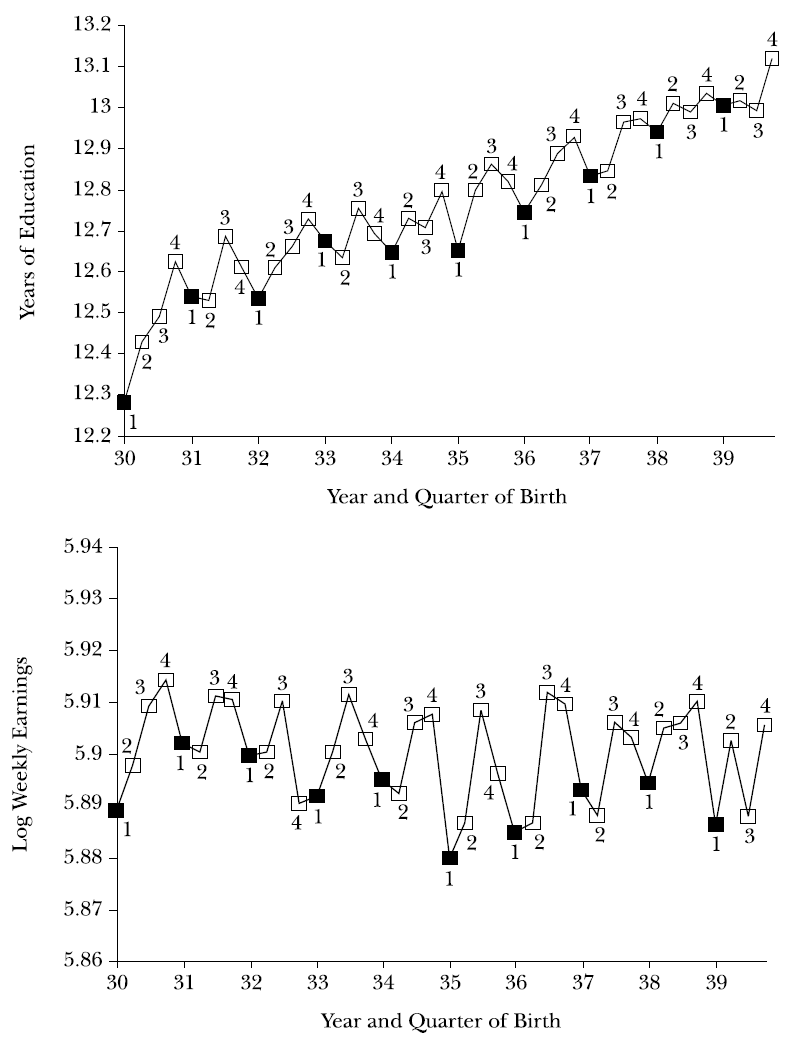
\includegraphics[width=0.65\linewidth, keepaspectratio]{Figuras/angrist-krueger-qob-educacion-salario-anotado.png} 
\end{figure}
\begin{itemize}
	\item 
\end{itemize}
\end{frame}	


\begin{frame}{Ejemplo: \citet{angrist_does_1991}}
	\begin{figure}[h!]
		\centering
		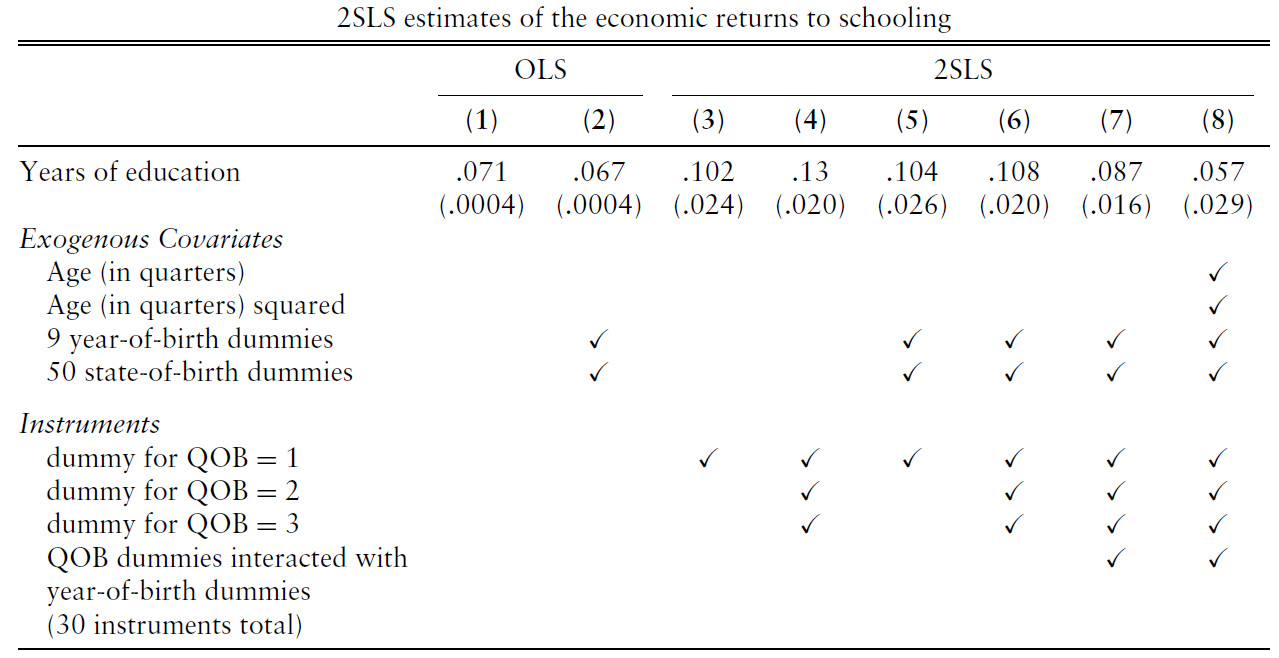
\includegraphics[width=0.95\linewidth, keepaspectratio]{Figuras/angrist-krueger-2sls-retornos-educacion.png} 
	\end{figure}
\end{frame}	


\begin{frame}{Instrumentos débiles}
\begin{itemize}
	\item Es fundamental que los instrumentos tengan una \textcolor{red}{\textbf{primera etapa fuerte}}. Consideremos el \textbf{caso más sencillo}: 
    \vspace{0.75em}
    \begin{enumerate}
        \item Una única variable explicativa ($D_i$).
        \item Variables normalizadas: $\EX[Y_i]=\EX[D_i]=\EX[e_i]=0$.
    \end{enumerate}
    %%\pause
    \smallspace
\begin{align*}
    \begin{split}
    Y_{i} = \brown{\tau}D_i + e_{i}; \qquad \EX[D_ie_i]\neq 0.
    \end{split}
\end{align*}
    %%\pause
    \item Supongamos un instrumento $\textcolor{blue}{z_i}$ tal que $\EX[\textcolor{blue}{z_i}]=0$ y $\EX[\textcolor{blue}{z_i}e_i]=0$. Premultiplicando por $\textcolor{blue}{z_i}$, tomando esperanzas y reorganizando:
    \begin{align*}
    \brown{\tau} = \frac{\EX[\textcolor{blue}{z_i} Y_i]}{\EX[\textcolor{blue}{z_i}D_i]}.
    \end{align*}
    \vspace{-0.75em}
    %%\pause
	\item En este caso, la primera etapa es:
    \vspace{-0.75em}
	\begin{align*}
	\begin{split}
	D_i = \textcolor{brown}{\theta} \textcolor{blue}{z_{i}} + \eta_{i}.
	\end{split}
	\end{align*}
\end{itemize}	
\end{frame}	


\begin{frame}{Instrumentos que no son relevantes}
\begin{itemize}
	\item \textbf{Caso extremo}: si $\textcolor{brown}{\theta}=0 \;\Rightarrow\; \EX[\textcolor{blue}{z_i}D_i]=0$, el estimador IV no está definido (asintóticamente). En \textbf{muestra finita}, el análogo muestral rara vez es exactamente cero, por lo que podemos calcular:
	\begin{align*}
	\begin{split}
	   \brown{\hat{\tau}_{IV}} = \frac{1/N\sum_{i=1} \textcolor{blue}{z_i} Y_i}{1/N\sum_{i=1} \textcolor{blue}{z_i} D_i}.
	\end{split}
	\end{align*}
    %%\pause
    \smallspace
	En estas condiciones, $\brown{\hat{\tau}_{IV}}$ puede ser \textbf{arbitrario}. Por eso es clave revisar la \textbf{significancia de los instrumentos en la primera etapa}.
\end{itemize}	
\end{frame}


\begin{frame}{Instrumento débil y endógeno}
\begin{itemize}
	\item Supongamos ahora que $\EX[\textcolor{blue}{z_i}e_i]\neq0$. El estimador IV se puede escribir como:
	\begin{align*}
    \begin{split}
    \brown{\hat{\tau}_{IV}} &= \brown{\tau} + \left(\frac{1}{N}\sum_{i=1} \textcolor{blue}{z_i} D_i\right)^{-1}\left(\frac{1}{N}\sum_{i=1} \textcolor{blue}{z_i} e_i\right).  \\
    \end{split}
    \end{align*}
    %%\pause
    \item Su probabilidad límite es:
	\begin{align*}
    \begin{split}
    \plim \brown{\hat{\tau}_{IV}} &= \brown{\tau} + \plim \left(\frac{1}{N}\sum_{i=1} \textcolor{blue}{z_i} D_i\right)^{-1} \plim \left(\frac{1}{N}\sum_{i=1} \textcolor{blue}{z_i} e_i\right)  \\
    &= \brown{\tau} + \frac{\EX[\textcolor{blue}{z_i}e_i]}{\EX[\textcolor{blue}{z_i} D_i]} \neq \brown{\tau}.
    \end{split}
    \end{align*}
	Si $\EX[\textcolor{blue}{z_i}e_i]\neq0$, la magnitud del sesgo depende de $\EX[\textcolor{blue}{z_i}D_i]$: \textbf{se magnifica el sesgo}.
\end{itemize}	
\end{frame}


%%%%%%%%%%%%%%%%%%%%%%%%%%%%%%%%%%%%%%%%%%%%%%%%%%%%%%%%%%%%%%%%%%%%%
%%%%%%%%%%%%%%%%%%%%%%%%%%%%%%%%%%%%%%%%%%%%%%%%%%%%%%%%%%%%%%%%%%%%%
\section{IV con efectos heterogéneos}
%%%%%%%%%%%%%%%%%%%%%%%%%%%%%%%%%%%%%%%%%%%%%%%%%%%%%%%%%%%%%%%%%%%%%

\begin{frame}{Efectos heterogéneos en IV}
\begin{itemize}
	\item Hemos interpretado el \textcolor{blue}{efecto causal} estimado por IV como si fuera homogéneo (igual para todas las unidades) o como un promedio (ya sea de la población o de los tratados).
		\begin{align*}
			\begin{split}
				\textcolor{brown}{\tau_{ATE}} &\equiv \EX[\underbrace{Y_i(1) - Y_i(0)}_{\textcolor{brown}{\equiv \tau_i}}] \\
				\textcolor{brown}{\tau_{ATT}} &\equiv \EX[\underbrace{Y_i(1) - Y_i(0)}_{\textcolor{brown}{\equiv \tau_i}}|D_i=1].
			\end{split}
		\end{align*}
    %%\pause
	\item ¿Qué estamos estimando cuando usamos IV?
\end{itemize}
\end{frame}


\begin{frame}{¿Qué estamos estimando?}
\begin{itemize}
	\item Es posible que el instrumento sólo ``afecte'' a un \textbf{subconjunto de la población}.
	\begin{figure}	
		\centering
		\begin{tikzpicture}[scale=2]	
		\node [left] at  (0.1,0) {$\textcolor{blue}{z_i}$};
		\node [left] at  (0.7,0) {$\textcolor{red}{D_i}$};	
		\node [right] at (1.2,0) {$Y_i$};
		\node [below] at (0.95,-0.35) {$e_i$};	
		\draw [->]       (0.1,0) -- (0.45,0);			
		\draw [->]       (0.7,0) -- (1.2,0);		
		\draw [->,dashed] (0.95,-0.35) -- (0.6,-0.1);
		\draw [->,dashed] (0.95,-0.35) -- (1.3,-0.1);
		\draw[fill] (0.1,-0) circle [radius =0.02];									
		\draw[fill] (0.7,-0) circle [radius =0.02];		
		\draw[fill] (0.95,-0.35) circle [radius =0.02];			
		\end{tikzpicture}	
	\end{figure}
	%%\pause
	\smallspace
	\begin{itemize}	
	\item En \citet{angrist_does_1991}, ¿qué estudiantes se ven afectados por el instrumento?
	%%\pause
	\smallspace
	    \item Un estudiante que no se quiere retirar del colegio no se ve afectado por la política $\rightarrow$ el trimestre de nacimiento no cambia su decisión.
	\end{itemize}    
\end{itemize}
\begin{enumerate}
    %%\pause
    \item Si el instrumento sólo afecta a un \textbf{subconjunto de la población}, el \textcolor{blue}{efecto causal} estimado aplica a esa \textcolor{blue}{subpoblación}.   
    %%\pause
    \item Si el efecto es \textcolor{blue}{heterogéneo} entre subpoblaciones, tenemos que tener cuidado con la forma como lo interpretamos.
\end{enumerate}  
\end{frame}


%%%%%%%%%%%%%%%%%%%%%%%%%%%%%%%%%%%%%%%%%%%%%%%%%%%%%%%%%%%%%%
\subsection{- Resultados potenciales}
%%%%%%%%%%%%%%%%%%%%%%%%%%%%%%%%%%%%%%%%%%%%%%%%%%%%%%%%%%%%%%

\begin{frame}{Ejemplo: \citet{Angrist1990}}
\begin{itemize}
	\item \textbf{Pregunta}: efecto de largo plazo de prestar servicio militar durante la guerra de Vietnam sobre el ingreso.
	\smallspace
	%%\pause
	\item \textbf{Endogeneidad} por autoselección:
	\begin{figure}	
		\begin{tikzpicture}[scale=2]	
		\node [left] at  (0.7,0) {\textcolor{red}{Veterano}};	
		\node [right] at (1.2,0) {Ing};
		\node [below] at (0.95,-0.35) {$e$};		
		\draw [->]       (0.7,0) -- (1.2,0);		
		\draw [->,dashed] (0.95,-0.35) -- (0.6,-0.1);
		\draw [->,dashed] (0.95,-0.35) -- (1.3,-0.1);						
		\draw[fill] (0.7,-0) circle [radius =0.02];		
		\draw[fill] (0.95,-0.35) circle [radius =0.02];			
		\end{tikzpicture}	
	\end{figure} 
	%%\pause
	\item \textbf{Instrumento:} resultado de una \textbf{lotería} que determinaba si una persona podía ser llamada a prestar servicio de manera obligatoria. 
	%%\pause
	\smallspace
	\begin{itemize}
		\item  Para personas de una cohorte determinada, se asignaban números aleatorios a cada fecha de nacimiento (números entre 1-365). \vspace{0.1cm} 
		%%\pause
		\item Todas las personas con un número menor a un valor especificado por el Departamento de Defensa de Estados Unidos eran elegibles. \vspace{0.1cm}
	\end{itemize}
\vspace{0.2cm}
	\begin{figure}	
		\begin{tikzpicture}[scale=2]	
		\node [left] at  (-0.5,0) {\textcolor{blue}{Lotería}};		
		\node [left] at  (0.7,0) {\textcolor{red}{Veterano}};	
		\node [right] at (1.2,0) {Ing};
		\node [below] at (0.95,-0.35) {$e$};		
		\draw [->]       (-0.5,0) -- (-0.05,0);	
		\draw [->]       (0.7,0) -- (1.2,0);		
		\draw [->,dashed] (0.95,-0.35) -- (0.6,-0.1);
		\draw [->,dashed] (0.95,-0.35) -- (1.3,-0.1);						
		\draw[fill] (-0.5,-0) circle [radius =0.02];		
		\draw[fill] (0.7,-0) circle [radius =0.02];		
		\draw[fill] (0.95,-0.35) circle [radius =0.02];			
		\end{tikzpicture}	
	\end{figure} 
\end{itemize}
\end{frame}


\begin{frame}{Condición de tratamiento}
	\begin{itemize}
		\item Instrumento:
    \begin{align*}
    \textcolor{blue}{z_i} = 
        \begin{cases}
        1 &\hspace{0.5pt} \text{si $i$ es elegible dado el resultado de la lotería},\\
        0 &\hspace{0.5pt} \text{de lo contrario}.
        \end{cases}
    \end{align*}		
    %%\pause
		\item Condición de veterano: 
\begin{align*}
    \textcolor{red}{D_i} = 
    \begin{cases}
    1 &\hspace{0.5pt} \text{si $i$ es veterano de la guerra de Vietnam},\\
    0 &\hspace{0.5pt} \text{de lo contrario}.
    \end{cases}
\end{align*}		
    %%\pause
		\item La condición de veterano puede estar afectada por el resultado de la lotería, pero \textbf{la relación no es determinística}. 
\begin{align*}
    \textcolor{red}{D_i} = 
    \begin{cases}
    D_i(1) &\hspace{0.5pt} \text{si $\textcolor{blue}{z_i}=1$},\\
    D_i(0) &\hspace{0.5pt} \text{si $\textcolor{blue}{z_i}=0$}.
    \end{cases}
\end{align*}		
	\end{itemize}
\end{frame}


\begin{frame}{Primera etapa}
\begin{itemize}
	\item La condición de veterano observada es: \\ 
	\vspace{-0.6cm}
	\begin{align*}
		\textcolor{red}{D_i} = D_i(0) + \Big(D_i(1)-D_i(0)\Big) \textcolor{blue}{z_i}.
	\end{align*}
    \vspace{-1.3em}
	%%\pause
	\item En términos de una regresión lineal: 
	\begin{align*}
	\textcolor{red}{D_i} = \underbrace{\gamma_0}_{\EX[D_i(0)]} + \underbrace{\textcolor{brown}{\gamma_{i1}}}_{(D_i(1)-D_i(0))} \textcolor{blue}{z_i} + \underbrace{\eta_i}_{D_i(0)-\EX[D_i(0)]}.    
	\end{align*}
    \vspace{-1.0em}
	%%\pause
	\item $\textcolor{brown}{\gamma_{i1}}$: \textcolor{blue}{efecto causal} (posiblemente \textcolor{blue}{heterogéneo}) de ser elegible sobre la condición de veterano de guerra. El \textcolor{blue}{efecto causal promedio} es $\EX[\textcolor{brown}{\gamma_{i1}}]=\EX[D_i(1)-D_i(0)]$. 
	\vspace{0.75em}
	%%\pause
	\item \textbf{Primera etapa} en MC2E, pero con \textcolor{blue}{efectos heterogéneos}.
	\smallspace
	\begin{figure}	
		\begin{tikzpicture}[scale=2]	
			\node [left] at  (-0.5,0) {\textcolor{blue}{Lotería}};		
			\node [left] at  (0.7,0) {\textcolor{red}{Veterano}};	
			\node [right] at (1.2,0) {Ing};
			\node [below] at (0.95,-0.35) {$e$};		
			\draw [->]       (-0.5,0) -- (-0.05,0);	
			\draw [->]       (0.7,0) -- (1.2,0);		
			\draw [->,dashed] (0.95,-0.35) -- (0.6,-0.1);
			\draw [->,dashed] (0.95,-0.35) -- (1.3,-0.1);						
			\draw[fill] (-0.5,-0) circle [radius =0.02];		
			\draw[fill] (0.7,-0) circle [radius =0.02];		
			\draw[fill] (0.95,-0.35) circle [radius =0.02];			
		\end{tikzpicture}	
	\end{figure}
\end{itemize}
\end{frame}


\begin{frame}{Resultados potenciales y efectos causales}
\begin{itemize}
	\item La variable de resultado es el ingreso $Y_i$.
	\item Hay que expandir la \textbf{notación} para pensar en resultados potenciales en términos tanto de la condición de veterano como del resultado de la lotería.
	%\pause
		\item \textbf{Resultados potenciales} para la variable de ingreso.
	\begin{align*}
	Y_i = 
		\begin{cases}
		Y_i(1,1) &\hspace{0.5pt} \text{si $\textcolor{red}{D_i}=1$ y $\textcolor{blue}{z_i} =1$}\\
		Y_i(1,0) &\hspace{0.5pt} \text{si $\textcolor{red}{D_i}=1$ y $\textcolor{blue}{z_i} =0$}\\
		Y_i(0,1) &\hspace{0.5pt} \text{si $\textcolor{red}{D_i}=0$ y $\textcolor{blue}{z_i} =1$}\\
		Y_i(0,0) &\hspace{0.5pt} \text{si $\textcolor{red}{D_i}=0$ y $\textcolor{blue}{z_i} =0$}
		\end{cases}
	\end{align*}	
\end{itemize}
\end{frame}


%%%%%%%%%%%%%%%%%%%%%%%%%%%%%%%%%%%%%%%%%%%%%%%%%%%%%%%%%%%%%%
\subsection{- Supuestos IV con efectos heterogéneos}
%%%%%%%%%%%%%%%%%%%%%%%%%%%%%%%%%%%%%%%%%%%%%%%%%%%%%%%%%%%%%%

\begin{frame}{Supuesto I: independencia}
	\begin{enumerate}
		\item[I.] \textcolor{blue}{Independencia.} El instrumento es independiente de los \textbf{resultados potenciales}, $Y_i(D,z)$, y los \textbf{potenciales estados de tratamiento}, $D_i(z)$: 		
        \vspace{-1em}
		\begin{align*}
		Y_i(1,1), Y_i(1,0), Y_i(0,1), Y_i(0,0),D_i(0), D_i(1) \indep \textcolor{blue}{z_i}. 
		\end{align*}			
	    En palabras, el instrumento es \textit{``as good as random''}. ¿Se cumple en nuestro ejemplo?
    \end{enumerate}
\begin{itemize}
\smallspace	
    %\pause	
	\item Permite recuperar el \textcolor{blue}{efecto causal promedio} del instrumento sobre la \textbf{variable de tratamiento}:	
	\begin{align*}
	\begin{split}
	\EX[\textcolor{red}{D_i}|\textcolor{blue}{z_i} =1] - \EX[\textcolor{red}{D_i}|\textcolor{blue}{z_i} =0] &=  \EX[D_i(1)|\textcolor{blue}{z_i} =1] - \EX[D_i(0)|\textcolor{blue}{z_i} =0]\\
	&= \EX[D_i(1) - D_i(0)] = \EX[\textcolor{brown}{\gamma_{i1}}]. 
	\end{split}
	\end{align*}
	%%\pause
	Se puede obtener corriendo una regresión de $\textcolor{red}{D_i}$ en $\textcolor{blue}{z_i} $ (primera etapa de MC2E).
\end{itemize}	
\end{frame}


\begin{frame}{Supuesto II: restricción de exclusión}
	\begin{enumerate}
		\item[II.] \textcolor{blue}{Restricción de exclusión.} 
		\begin{align*}
			Y_i(D,1) = Y_i(D,0) = Y_i(D) \quad \text{para} \quad D \in \{0,1\}. 
		\end{align*}
        En palabras, los resultados potenciales, $Y_i(D,z)$, sólo dependen de la condición de veterano $D$, no del valor del instrumento.
	\end{enumerate}
	\begin{figure}	
	\begin{tikzpicture}[scale=2]	
	\node [left] at  (-0.5,0) {\textcolor{blue}{Lotería}};		
	\node [left] at  (0.7,0) {\textcolor{red}{Veterano}};	
	\node [right] at (1.2,0) {Ing};
	\node [below] at (0.95,-0.35) {$e$};		
	\draw [->]       (-0.5,0) -- (-0.05,0);	
	\draw [->]       (0.7,0) -- (1.2,0);		
	\draw [->,dashed] (0.95,-0.35) -- (0.6,-0.1);
	\draw [->,dashed] (0.95,-0.35) -- (1.3,-0.1);						
	\draw[fill] (-0.5,-0) circle [radius =0.02];		
	\draw[fill] (0.7,-0) circle [radius =0.02];		
	\draw[fill] (0.95,-0.35) circle [radius =0.02];			
	\end{tikzpicture}	
\end{figure}	
%\pause
\begin{itemize}
	\item Suponga que se cumple el \textcolor{blue}{supuesto de independencia}, piense en un ejemplo en el que la \textcolor{blue}{restricción de exclusión} no se cumple. 
\end{itemize}
\end{frame}


\begin{frame}{Supuesto II: restricción de exclusión}
\begin{itemize}
	\item El supuesto implica que podemos relajar la notación: 
	\begin{align*}
	\begin{split}
	Y_i(1) = Y_i(1,1) = Y_i(1,0)	\\
	Y_i(0) = Y_i(0,1) = Y_i(0,0) 
	\end{split}
	\end{align*}
    %\pause
    \item El \textbf{ingreso observado} es:
	\begin{align*}
	\begin{split}
	Y_i = Y_i(0) + \Big(Y_i(1)-Y_i(0)\Big)\textcolor{red}{D_i}. \\
	\end{split}
	\end{align*}
	%\pause
    En términos de una regresión:
	\begin{align*}
	Y_i = \underbrace{\beta_0}_{\EX[Y_i(0)]} + \underbrace{\textcolor{brown}{\tau_{i}}}_{(Y_i(1)-Y_i(0))} \textcolor{red}{D_i} + \underbrace{e_i}_{Y_i(0)-\EX[Y_i(0)]}   
	\end{align*}
	El parámetro $\textcolor{brown}{\tau_{i}}$ es el \textcolor{blue}{efecto causal} (posiblemente \textcolor{blue}{heterogéneo}) de ser veterano de guerra sobre el ingreso.
\end{itemize}
\end{frame}


\begin{frame}{Supuesto III: relevancia del instrumento}
	\begin{enumerate}
		\item[III.] \textcolor{blue}{Relevancia del instrumento.} 
		\end{enumerate}	
	\begin{itemize}
		\item Recordar que la primera etapa es
		\begin{align*}
		\textcolor{red}{D_i} = \underbrace{\gamma_0}_{\EX[D_i(0)]} + \underbrace{\textcolor{brown}{\gamma_{i1}}}_{(D_i(1)-D_i(0))} \textcolor{blue}{z_i}+ \underbrace{\eta_i}_{D_i(0)-\EX[D_i(0)]}.    
		\end{align*}
	    Igual que en el modelo con \textbf{efectos constantes}, se requiere que $\EX[D_i(1)-D_i(0)]=\EX[\textcolor{brown}{\gamma_{i1}}]\neq0$.
	\end{itemize}	 
\end{frame}


\begin{frame}{Supuesto IV: monotonicidad}
	\begin{enumerate}
		\item[IV.] \textcolor{blue}{Monotonicidad} \citep{Imbens94}: 
		\begin{align*}
		D_i(1) - D_i(0) =\textcolor{brown}{\gamma_{i1}}\geq0 \quad \forall i \quad \text{ó} \quad D_i(1) - D_i(0) = \textcolor{brown}{\gamma_{i1}}\leq0 \quad \forall i
		\end{align*} 
	\end{enumerate}
    %\pause
	\begin{itemize}
		\item 	Es posible que para algunos individuos la condición de tratamiento \textbf{no se vea afectada por el instrumento} ($\textcolor{brown}{\gamma_{i1}}=0$), pero para \textbf{aquellos que sí son afectados, el efecto va en la misma ``dirección''}.	
	\end{itemize} 
\end{frame}


\begin{frame}{Supuesto IV: monotonicidad}
	\begin{itemize}
		\item Podemos dividir a la población en cuatro grupos: \\ \vspace{0.2cm}	
	\begin{center}
		\begin{tabular}{ | l | c | c |}
			\hline
			& $D_i(0)=0$ & $D_i(0)=1$ \\ \hline		
			$D_i(1)=0$ & \textcolor{blue}{nunca-tratado} & \textcolor{blue}{\textit{defier}} \\ \hline
			$D_i(1)=1$ & \textcolor{blue}{\textit{complier}} & \textcolor{blue}{siempre-tratado} \\ \hline
		\end{tabular}
	\end{center}
\mediumspace
	\begin{enumerate}
	\fontvid
	%\pause
		\item \textcolor{blue}{Nunca-tratado}: personas con incapacidades físicas u otras razones que les impide enlistarse en las Fuerzas Armadas. 
		%\pause
		\item \textcolor{blue}{Siempre-tratado}: personas que quieren enlistarse en las Fuerzas Armadas voluntariamente.
		%\pause
		\item \textcolor{blue}{Complier}: personas que se enlistan si salen elegibles, pero no se enlistan si no salen elegibles. De forma más general, es el \textbf{grupo para el cual el instrumento actúa en la ``dirección'' esperada.}
		%\pause
		\item \textcolor{blue}{Defier}: personas que se enlistan si no salen elegibles, pero no se enlistan si salen elegibles. De forma más general, es el \textbf{grupo para el cual el instrumento actúa en la ``dirección'' contraria a lo que se espera.}	
	\end{enumerate}
	\smallspace
	%\pause
\item \textcolor{red}{\textbf{El supuesto de monotonicidad implica que no hay \textit{defiers} en la población}.}
	\end{itemize}
 \end{frame}


 %%%%%%%%%%%%%%%%%%%%%%%%%%%%%%%%%%%%%%%%%%%%%%%%%%%%%%%%
\subsection{- Estimador de Wald}
%%%%%%%%%%%%%%%%%%%%%%%%%%%%%%%%%%%%%%%%%%%%%%%%%%%%%%%%

\begin{frame}{Estimador de Wald - identificación}
\begin{itemize} 
    \item Considere el modelo de regresión (cambiando \(\textcolor{brown}{\tau_i}\) por \(\textcolor{brown}{\tau}\)):
		\begin{align*}
		Y_i = \beta_0 + \textcolor{brown}{\tau} \textcolor{red}{D_i} + e_i; \,\, \text{donde} \,\,  \EX[e_i \vert \textcolor{blue}{z_i}]=0.
		\end{align*}
		%\pause
		\item Sacando el valor esperado condicional en $\textcolor{blue}{z_i}$,
		\begin{align*}
        \begin{split}
		\EX[Y_i|\textcolor{blue}{z_i}=1] &= \beta_0 + \textcolor{brown}{\tau} \EX[\textcolor{red}{D_i}|\textcolor{blue}{z_i}=1] \\
		\EX[Y_i|\textcolor{blue}{z_i}=0] &= \beta_0 + \textcolor{brown}{\tau} \EX[\textcolor{red}{D_i}|\textcolor{blue}{z_i}=0]
	\end{split}	
        \end{align*}
        %\pause
        \item Resolviendo para \(\textcolor{brown}{\tau}\):
		\begin{align*}
		\begin{split}
		\textcolor{brown}{\tau} = \frac{\EX[Y_i|\textcolor{blue}{z_i}=1] - \EX[Y_i|\textcolor{blue}{z_i}=0]}{\EX[\textcolor{red}{D_i}|\textcolor{blue}{z_i}=1] - \EX[\textcolor{red}{D_i}|\textcolor{blue}{z_i}=0]}.	
		\end{split}		
		\end{align*}
		El análogo muestral se conoce como el \textbf{estimador de Wald}. Es el mismo estimador IV o 2SLS con instrumento binario.
	\end{itemize}	
\end{frame}


%%%%%%%%%%%%%%%%%%%%%%%%%%%%%%%%%%%%%%%%%%%%%%%%%%%%%%%%%%%%%%
\subsection{- Interpretación LATE de IV}
%%%%%%%%%%%%%%%%%%%%%%%%%%%%%%%%%%%%%%%%%%%%%%%%%%%%%%%%%%%%%%

\begin{frame}{Interpretación LATE de variables instrumentales}\label{SLIDE:TEOR-LATE}
\begin{tcolorbox}[colback=white, title=Teorema LATE, arc=0mm,boxrule=0.5pt, breakable]
	Bajo los supuestos I-IV,
    {\small
    \begin{align*}
    \begin{split}
    \textcolor{brown}{\tau} = \frac{\EX[Y_i|\textcolor{blue}{z_i} =1] - \EX[Y_i|\textcolor{blue}{z_i} =0]}{\EX[\textcolor{red}{D_i}|\textcolor{blue}{z_i} =1] - \EX[\textcolor{red}{D_i}|\textcolor{blue}{z_i} =0]} &= \EX[Y_i(1)-Y_i(0)|D_i(1) - D_i(0) > 0] \\
    &= \EX[\textcolor{brown}{\tau_i}|\textcolor{brown}{\gamma_{i1}}>0]. 	
    \end{split}	
    \end{align*}	
}
\end{tcolorbox}
\begin{itemize}
    %\pause
    \item Ver demostración en el \hyperlink{ANEX:TEOR-LATE}{{\beamerreturnbutton{anexo}}}
    \item Este efecto lo llamamos ``\textcolor{blue}{local average treatment effect}'' (\textcolor{blue}{LATE}).
    %\pause
    \item \textcolor{blue}{LATE} es el efecto promedio de $\textcolor{red}{D_i}$ en $Y_i$ \textbf{para aquellas personas cuya condición de tratamiento puede cambiar por la influencia del instrumento ($\textcolor{blue}{z_i}$)}.
\end{itemize}
\end{frame}


\begin{frame}{Supuesto de monotonicidad (cont.)}
\begin{itemize}\setlength{\itemsep}{1.0em}
    \item El \textcolor{blue}{supuesto de monotonicidad} excluye la existencia de \textit{\textcolor{blue}{defiers}}: personas para las que $D(1)<D(0)$. %\pause
    \smallspace
    \begin{itemize}\setlength{\itemsep}{0.6em}
        \item Si hay \textcolor{blue}{defiers}, el instrumento mueve a algunos \textcolor{blue}{compliers} hacia el tratamiento y a algunos \textcolor{blue}{defiers} fuera de él. %\pause
        \smallskip
            \item Aun si \(\textcolor{brown}{\tau_i}=Y_i(1)-Y_i(0)>0\) para todos los \(i\), el estimador IV/Wald no necesariamente es positivo:
        \[
        \textcolor{brown}{\tau} = \frac{\EX[Y_i|\textcolor{blue}{z_i} =1] - \EX[Y_i|\textcolor{blue}{z_i} =0]}{\EX[\textcolor{red}{D_i}|\textcolor{blue}{z_i} =1] - \EX[\textcolor{red}{D_i}|\textcolor{blue}{z_i} =0]} =
        \frac{\Pr(c)\,\EX[\textcolor{brown}{\tau_i}\mid c] \;-\; \Pr(d)\,\EX[\textcolor{brown}{\tau_i}\mid d]}{\Pr(c)-\Pr(d)}.
        \]
        donde \(\Pr(c)\) y \(\Pr(d)\) son las fracciones de \textit{compliers} y \textit{defiers}, respectivamente. %\pause
        \smallskip
        \item \textbf{Intuición}: los \textcolor{blue}{defiers} entran con \emph{signo negativo} en el numerador; si \(\Pr(d) \neq 0\), el cociente puede ser negativo.
    \end{itemize}
\end{itemize}
\end{frame}


\begin{frame}{LATE, ATT y ATE}
\begin{itemize}
	\item Considere tres posibles efectos:
	\begin{equation*}
	\begin{split}
	\textcolor{brown}{\tau_{LATE}} &= \EX[Y_i(1) - Y_i(0)|\textcolor{blue}{complier}] \\ 
	\textcolor{brown}{\tau_{ATT}} &= \EX[Y_i(1) - Y_i(0)|D_i=1] \\
	\textcolor{brown}{\tau_{ATE}} &= \EX[Y_i(1) - Y_i(0)] \\ 
	\end{split}
	\end{equation*}	
	%\pause
	\item Identificando la población tratada:
	\begin{align*}
	\{\textcolor{red}{D_i}=1\} = \underbrace{\{D_i(0)=D_i(1)=1\}}_{\textcolor{blue}{siempre-tratado}} \cup \underbrace{\{\{D_i(1)>D_i(0)\}\cap \{\textcolor{blue}{z_i} =1\}\}}_{\text{\textcolor{blue}{\textit{complier}} con} \; \textcolor{blue}{z_i} =1} 
	\end{align*}
	$\textcolor{brown}{\tau_{LATE}}\neq\textcolor{brown}{\tau_{ATT}}$ a menos que no haya nadie en el grupo de \textcolor{blue}{siempre-tratados}. 
\end{itemize}	
\end{frame}


\begin{frame}{Validez interna y externa}	
\begin{itemize}\setlength{\itemsep}{1.0em}
	\item Bajo los supuestos descritos, el estimador que se obtiene por variables instrumentales tiene \textcolor{blue}{validez interna}: estima el efecto causal \textbf{para un grupo determinado de la población}. \\ \vspace{0.3cm}   
	%\pause
	\item \textbf{¿Podemos generalizar a otros contextos?} \\ \vspace{0.2cm} 
    %\pause   	
	\item Si hay efectos \textcolor{blue}{heterogéneos}, \textbf{diferentes instrumentos pueden resultar en diferentes efectos causales estimados, cada uno ``bien identificado''}. Esto se da porque la población de \textcolor{blue}{compliers} se define en función del instrumento. \\ \vspace{0.1cm}
\end{itemize}
\end{frame}


\begin{frame}{Ejemplo: \citet{Angrist1990}}
	\begin{figure}[h!]
		\centering
		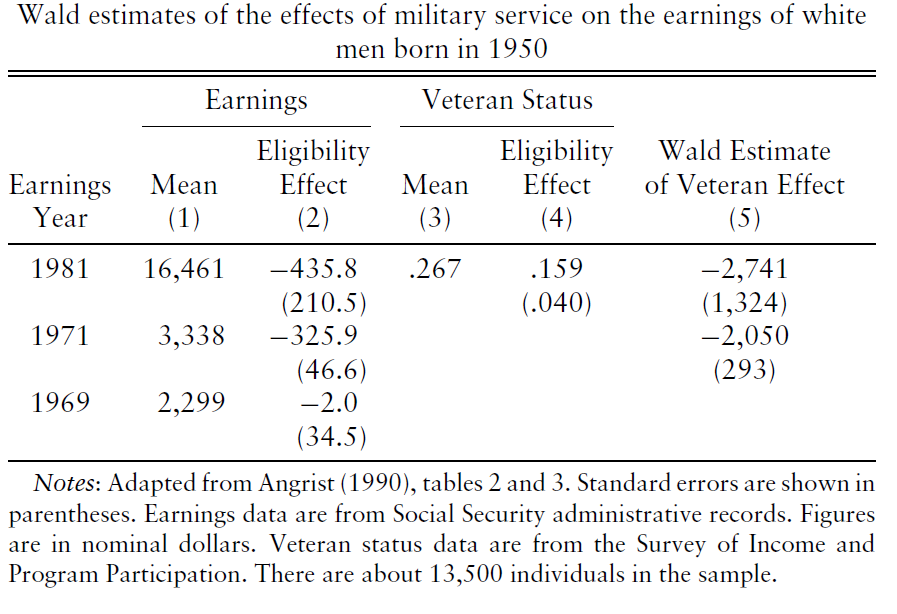
\includegraphics[width=0.7\linewidth, keepaspectratio]{Figuras/angrist1990-veteranos-vietnam-loteria.png} 
	\end{figure}
	\begin{itemize}
		\item Caída en el ingreso de aproximadamente 16.6\%.
	\end{itemize}
\end{frame}

%%%%%%%%%%%%%%%%%%%%%%%%%%%%%%%%%%%%%%%%%%%%%%%%%%%%%%%%%%%%%%
\section{RCTs con cumplimiento imperfecto}
%%%%%%%%%%%%%%%%%%%%%%%%%%%%%%%%%%%%%%%%%%%%%%%%%%%%%%%%%%%%%%

\begin{frame}{Aleatorización y decisión de participar}
\begin{itemize}\setlength{\itemsep}{1.0em}
    \item La variable $\textcolor{red}{D_i}\in \{0,1\}$ nos indica si la unidad $i$ recibió ($\textcolor{red}{D_i}=1$) o no ($\textcolor{red}{D_i}=0$) el tratamiento.
    \item En muchos contextos, \textbf{participar o no en un programa es una decisión}: 
    \begin{itemize}
        \item No se puede obligar a las personas a recibir un tratamiento.
        \item No se puede obligar a las personas a no recibir un tratamiento.
    \end{itemize}
    %\pause
    \item Si hay \textit{``imperfect compliance''} o \textit{``partial compliance''}, la \textbf{aleatorización no es el único determinante de la participación}. 
\end{itemize}	
\end{frame}


\begin{frame}{Aleatorización y decisión de participar}
	\begin{itemize}\setlength{\itemsep}{1.0em}
		\item Sea $\textcolor{blue}{z_i}\in \{0,1\}$ una variable indicadora de \textbf{asignación (aleatoria) al tratamiento}.
        \vspace{0.5em}
		\begin{enumerate}
			\item Hay personas para las cuales $\textcolor{blue}{z_i} =1$ pero no participan (\(\textcolor{red}{D_i}= 0\)).
			\item Hay personas para las cuales $\textcolor{blue}{z_i} =0$ pero sí participan (\(\textcolor{red}{D_i}= 1\)). \vspace{0.1cm}	
		\end{enumerate}
        En particular:
		\begin{align*}
		\Pr[\textcolor{red}{D_i}= 1|\textcolor{blue}{z_i} =1] \neq 1 \quad \text{y} \quad \Pr[\textcolor{red}{D_i}= 0|\textcolor{blue}{z_i} =0] \neq 1 
		\end{align*}
		%\pause
		\item \textbf{¿Qué factores determinan la decisión de participación?}
		\begin{itemize}
            \item Es factible que los que participan lo hacen porque el beneficio esperado de participar es mayor al de no hacerlo, generando un  \textcolor{blue}{problema de selección}: ($ Y_i(1),Y_i(0) \not\!\perp\!\!\!\perp \textcolor{red}{D_i}$). 
        \end{itemize}
	\end{itemize}	
\end{frame}


\begin{frame}{Asignación aleatoria como instrumento}
	\begin{itemize}
		\item Podemos \textbf{usar la asignación aleatoria como instrumento} de la decisión de participar.
		\begin{figure}	
			\centering
			\begin{tikzpicture}[scale=2]	
			\node [left] at  (0.1,0) {$\textcolor{blue}{z_i} $};
			\node [left] at  (0.7,0) {$\textcolor{red}{D_i}$};	
			\node [right] at (1.2,0) {$Y_i$};
			\node [below] at (0.95,-0.35) {$e_i$};	
			\draw [->]       (0.1,0) -- (0.45,0);			
			\draw [->]       (0.7,0) -- (1.2,0);		
			\draw [->,dashed] (0.95,-0.35) -- (0.6,-0.1);
			\draw [->,dashed] (0.95,-0.35) -- (1.3,-0.1);
			\draw[fill] (0.1,-0) circle [radius =0.02];									
			\draw[fill] (0.7,-0) circle [radius =0.02];		
			\draw[fill] (0.95,-0.35) circle [radius =0.02];			
			\end{tikzpicture}	
		\end{figure}		
		%\pause
		\item Si se cumplen los supuestos I-IV, el estimador por variables instrumentales tiene una \textbf{interpretación} \textcolor{blue}{LATE}.
		%\pause		
		\item Si el programa está \textbf{restringido a las personas que son asignadas al tratamiento} ($\Pr[D_i=1|\textcolor{blue}{z_i} =0]=0$), el estimador también tiene una interpretación \textcolor{blue}{ATT} (no hay un grupo de \textcolor{blue}{siempre-tratados}).
	\end{itemize}	
\end{frame}


\begin{frame}{Intención de tratamiento (ITT)}
\begin{itemize}\setlength{\itemsep}{1.0em}
	\item Considere el modelo en forma reducida:
	\begin{equation*}
	Y_i = \gamma_0 + \textcolor{brown}{\phi_{i1}} \textcolor{blue}{z_i}+ \mu_i
	\end{equation*}
	En este caso, comparamos personas dependiendo de si les \textbf{ofrecieron} el tratamiento, independiente de si lo reciben o no (sin considerar $\textcolor{red}{D_i}$).
	\pause
	\item Bajo los supuestos I-IV, podemos identificar $\EX[\textcolor{brown}{\phi_{i1}}]$. La interpretación del efecto estimado se conoce como \textcolor{blue}{``Intention to Treat''} ($\textcolor{blue}{ITT}$): el \textcolor{blue}{efecto causal} de ofrecer el tratamiento.
\end{itemize}	
\end{frame}


%%%%%%%%%%%%%%%%%%%%%%%%%%%%%%%%%%%%%%%%%%%%%%%%%%%%%%%%%%%%%%
\section{Regresión Discontinua Borrosa (RDB)}
%%%%%%%%%%%%%%%%%%%%%%%%%%%%%%%%%%%%%%%%%%%%%%%%%%%%%%%%%%%%%%

\begin{frame}{Regresión Discontinua (RD) - reglas de asignación}
\begin{itemize}\setlength{\itemsep}{1.0em}
	\item En RD ``nítida'' (RDN), usamos la \textit{arbitrariedad} de ciertas \textcolor{blue}{reglas de asignación} \textbf{en el margen} para estimar el efecto causal. \vspace{0.1cm}
	\pause
	\item Notación: \vspace{0.1cm}
	\begin{itemize}\setlength{\itemsep}{0.7em}
		\item $Z_i$: \textit{running variable} que determina la \textcolor{red}{\textbf{elegibilidad}} al tratamiento (\textit{e.g.}, instrumento de focalización, puntaje en la prueba, \textit{etc}). 
		\item $\textcolor{red}{Z_0}$: \textbf{umbral} de elegibilidad (conocido). 
		\item $D_i = \mathbf{1}\{\text{si recibe el tratamiento}\}$. 
		\item $Y_i$: variable de resultado.
	\end{itemize}
\end{itemize}
\end{frame}


\begin{frame}{Implicaciones de los supuestos de RDN}
\begin{itemize}
 		\item En RDN, si sabemos el valor de $Z_i$, sabemos el valor de $D_i$: es una función determinística:
	\begin{align*}
		D_i = 
		\begin{cases}
			1 & \text{si } Z_i \geq \textcolor{red}{Z_0},\\
			0 & \text{si } Z_i < \textcolor{red}{Z_0}. 	
		\end{cases}
	\end{align*}
    \begin{figure}
        \begin{tikzpicture}[scale=1.3] % Increased scale for better visibility
        \draw[thick,->] (0,1) -- (5,1) node[right] {$Z_i$}; % Extend and label the axis
        \draw[thick,->] (0,1) -- (0,3.5) node[above] {\footnotesize $\Pr[D_i = 1 \vert Z_i]$}; % Extend and label the Y-axis    
        % Adjusted and more prominent lines
        \draw [ultra thick] (0,1)--(2,1); % Base level line
        \draw [ultra thick, red] (2,3)--(4.5,3); % Elevated level line
        \draw [dashed, thick] (2,1)--(2,3); % Dashed line for discontinuity    
        % Base and top dotted lines for reference
        \draw [dotted] (0,1)--(4.5,1); % Base level dotted line
        \draw [dotted] (0,3)--(4.5,3); % Top level dotted line    
        % Labels and nodes
        \node [left] at (0,1) {$0$};
        \node [left] at (0,3) {$1$};
        \node [below] at (2,0.9) {\textcolor{red}{$Z_0$}};    
        % Highlighting the cutoff point
        \draw[fill=red] (2,3) circle [radius=0.1]; % Emphasized cutoff point
        \draw (2,1) circle [radius=0.1]; % Base circle    
        \end{tikzpicture}
    \end{figure}
\end{itemize}
\end{frame}



\begin{frame}{Regresión Discontinua Borrosa (RDB)}
    \begin{itemize}\setlength{\itemsep}{1.0em}
        \item En \textbf{RDB} relajamos el supuesto de cumplimiento perfecto (\textit{``perfect compliance''}).  
        \pause
        \item \textcolor{red}{\textbf{Requisito clave}}: \textbf{salto} en la probabilidad de tratamiento en el umbral:
        \begin{align*}
            \lim_{z \to \textcolor{red}{Z_0}^-} \Pr\left[D_i=1|Z_i = z\right] \neq \lim_{z \to \textcolor{red}{Z_0}^+} \Pr\left[D_i=1| Z_i = z\right].
        \end{align*}
        \pause
        De forma general, si 
        \[
            \Pr[D_i=1|Z_i] = g(Z_i),
        \] 
        podemos ser agnósticos sobre la forma funcional de \(g(\cdot)\), pero la probabilidad debe ``saltar'' en el umbral $\textcolor{red}{Z_0}$. 
    \end{itemize}	
\end{frame}


\begin{frame}{Ejemplo}
\begin{figure}
	\begin{tikzpicture}[scale=1.3]	
	\draw[thick,->] (0,0) -- (4.3,0);	
	\draw[thick,->] (0,0) -- (0,3.3);	
	\draw [thick] (0,0.5)--(2,0.7);
	\draw [dashed] (2,0.7)--(2,1.8);
	\draw [thick, red] (2,1.8)--(4.3,2.7);
	\draw [dotted] (0,3)--(4.3,3);		
	\node [left] at (0,0.0) {$0$};	
	\node [below] at (2,0) {$\textcolor{red}{Z_0}$};	
	\node [below] at (4.3,0) {$Z_i$};	
	\node [left] at (0,3) {$1$};	
	\node [above] at (0,3.3) {\footnotesize $\Pr[D_i = 1 \vert Z_i] = g(Z_i)$};
	\draw[fill, red] (2,1.8) circle [radius =0.05];		
	\draw (2,0.7) circle [radius =0.05];	
	\end{tikzpicture}
\end{figure}
\begin{itemize}
    \pause
	\item La asignación deja de ser determinística: factores observados/no observados influyen en $D_i$.
\end{itemize}
\end{frame}


\begin{frame}{Ecuación de interés}
	\begin{itemize}
		\item La ecuación de interés es la misma que derivamos en el caso de RDN: \vspace{-0.2cm}
	\begin{align*}
		Y_i = m(Z_i) + \textcolor{brown}{\tau(Z_i)} D_i + e_i
	\end{align*}	
    donde
    \begin{itemize}\setlength{\itemsep}{0.7em}
        \item \(m(Z_i) \equiv \EX[Y_i(0)|Z_i]\) es la CEF en \textbf{ausencia de tratamiento}.
        \item \(\textcolor{brown}{\tau(Z_i)} \equiv \EX[Y_i(1)-Y_i(0)|Z_i]\) es el \textbf{CATE}.
    \end{itemize}
	\end{itemize}	
\end{frame}


\begin{frame}{Primera etapa}
\begin{itemize}\setlength{\itemsep}{0.75em}
    \item Defina el instrumento \(\textcolor{blue}{Z_i^*}=\mathbf{1}\{Z_i\ge \textcolor{red}{Z_0}\}\).
    \pause
    \item \textbf{Primera etapa}:
    {\small
  \begin{align*} 
  \begin{split}     
    g(Z_i) &= g_-(Z_i) (1-\textcolor{blue}{Z_i^*}) + g_+(Z_i)\,\textcolor{blue}{Z_i^*} \\
           &= g_-(Z_i) + \underbrace{\Big(g_+(Z_i)-g_-(Z_i)\Big)}_{\brown{\pi(Z_i)}}\,\textcolor{blue}{Z_i^*}.
  \end{split}
  \end{align*}
  }
    donde \(g_-(Z_i)\) (\(g_+(Z_i)\))  es la probabilidad de recibir el tratamiento a la izquierda (derecha) del punto de corte.
	\pause
	\item Si no hay manipulación del \emph{running variable}, las covariables (observadas y no observadas) deberían estar balanceadas \textbf{en la vecindad} de $\textcolor{red}{Z_0}$ y \(\textcolor{blue}{Z_i^*}\) es un instrumento válido.
	\pause
	\item  \textbf{Monotonicidad local}: cruzar el umbral no reduce la probabilidad de tratamiento para ninguna unidad en la vecindad de $\textcolor{red}{Z_0}$.
\end{itemize}	
\end{frame}


\begin{frame}{Ecuación estructural y primera etapa}
    \begin{itemize}
        \item \textbf{Ecuación de interés}: \vspace{-0.3cm}
        \begin{align*}
            Y_i = m(Z_i) + \textcolor{brown}{\tau(Z_i)} D_i + e_i
        \end{align*}
	\item \textbf{Primera etapa}: \vspace{-0.3cm}
	\begin{align*}
	   D_i = g_-(Z_i) + \textcolor{brown}{\pi(Z_i)} \textcolor{blue}{Z^*_i} + \eta_i,
	\end{align*}
	La magnitud del salto en la probabilidad en el umbral de elegibilidad, capturado por $\textcolor{brown}{\pi}$, nos indica la ``fuerza'' de la primera etapa.
	\end{itemize}	
\end{frame}


\begin{frame}{Identificación}
\begin{itemize}\setlength{\itemsep}{1em}    
    \item En RDB el efecto identificado es un \textcolor{blue}{LATE local en el umbral}: el efecto sobre las unidades cuya condición de tratamiento cambia al cruzar \(\textcolor{red}{Z_0}\) (compliers locales).
    \pause
    \item \textbf{Wald local (no paramétrico):}
    \begin{align*}
        \textcolor{brown}{\tau} = \frac{\lim_{z \to \textcolor{red}{Z_0}^+} \EX\left[Y_i|Z_i = z\right] - \lim_{z \to \textcolor{red}{Z_0}^-} \EX\left[Y_i| Z_i = z\right]}{\lim_{z \to \textcolor{red}{Z_0}^+} \EX\left[D_i|Z_i = z\right] - \lim_{z \to \textcolor{red}{Z_0}^-} \EX\left[D_i| Z_i = z\right]}.
    \end{align*}	
    \pause
    \item \textbf{Estimación práctica:} MC2E con regresiones locales a cada lado del umbral y un ancho de banda. 
    \pause
    \item Dado el supuesto de continuidad en la vecindad de $\textcolor{red}{Z_0}$ y no manipulación, aplican los mismos métodos para verificar supuestos que en RDN.
\end{itemize}
\end{frame}


%%%%%%%%%%%%%%%%%%%%%%%%%%%%%%%%%%%%%%%%%%%%%%%%%%%%%%%%%%%%%%
%Anexos
%%%%%%%%%%%%%%%%%%%%%%%%%%%%%%%%%%%%%%%%%%%%%%%%%%%%%%%%%%%%%%

\section{Anexos}

\begin{frame}{Estimador IV y MC2E}\label{DIAP:DEMOS-MC2E}
\begin{itemize}
    \item Definimos el vector de instrumentos \(\textcolor{blue}{\ZB_i} = (\textcolor{blue}{z_i}, \WB_i)\) de dimensión $K \times 1$. Para la muestra completa, $\textcolor{blue}{\ZB}$ es una matriz $N \times K$.
    \smallspace
    \item La proyección de las regresoras $\XB = (D, \WB)$ sobre el espacio generado por los instrumentos es:
    \[
        \textcolor{blue}{\hat{\XB}} = \textcolor{blue}{\ZB} (\textcolor{blue}{\ZB}'\textcolor{blue}{\ZB})^{-1}\textcolor{blue}{\ZB}'\XB 
        = \textcolor{blue}{\textbf{P}_Z}\,\XB,
    \]
    donde $\textcolor{blue}{\textbf{P}_Z}$ es la \textbf{matriz de proyección} sobre el espacio de los instrumentos.    
    \vspace{0.3cm}
    \item Dimensiones:
    \begin{itemize}
        \item $\XB$: matriz $N \times K$ de regresores (incluye $D_i$ y controles).
        \item $\textcolor{blue}{\ZB}$: matriz $N \times K$ de instrumentos.
        \item $\textcolor{blue}{\hat{\XB}}$: matriz $N \times K$ de regresores proyectados.
    \end{itemize}
\end{itemize}
\end{frame}


\begin{frame}{Estimador IV y MC2E}
\begin{itemize}
\item $\textcolor{blue}{\textbf{P}_Z}$ es simétrica ($\textcolor{blue}{\textbf{P}_Z}=\textcolor{blue}{\textbf{P}'_Z}$) e idempotente ($\textcolor{blue}{\textbf{P}_Z}\textcolor{blue}{\textbf{P}_Z}=\textcolor{blue}{\textbf{P}_Z}$).
\begin{align*}
\begin{split}
\betaBH_{IV} &= (\textcolor{blue}{\hat{\XB}}'\XB)^{-1}\textcolor{blue}{\hat{\XB}}'\yB \\
&= \Big((\textcolor{blue}{\textbf{P}_Z} \XB)'\XB\Big)^{-1}\textcolor{blue}{\hat{\XB}}'\yB \\
&= \Big( \XB'\textcolor{blue}{\textbf{P}_Z}\XB\Big)^{-1}\textcolor{blue}{\hat{\XB}}'\yB \\ 
&= \Big((\textcolor{blue}{\textbf{P}_Z} \XB)' \textcolor{blue}{\textbf{P}_Z}\XB\Big)^{-1}\textcolor{blue}{\hat{\XB}}'\yB \\
&= \Big(\textcolor{blue}{\hat{\XB}}'\textcolor{blue}{\hat{\XB}}\Big)^{-1}\textcolor{blue}{\hat{\XB}}'\yB \\
\end{split}
\end{align*}
\item El estimador IV es equivalente al que se obtendría al estimar la siguiente regresión (\textcolor{blue}{segunda etapa}) por MCO \vspace{-0.0cm}
\begin{align*}
\begin{split}
Y_{i} &= \textcolor{blue}{\hat{\XB}}'_i\betaB + \mu_{i}, \\
\end{split}
\end{align*}	
donde $\mu_i \equiv e_i + (\XB_i - \textcolor{blue}{\hat{\XB}_i})'\betaB$. \hyperlink{DIAP:MC2E}{{\beamerreturnbutton{Regresar}}}
\end{itemize}
\end{frame}	



\begin{frame}{El teorema LATE I}\label{ANEX:TEOR-LATE}
\begin{itemize}
    \item Queremos demostrar que:
    \begin{align*}
\begin{split}
\textcolor{brown}{\tau} = \frac{\EX[Y_i|\textcolor{blue}{z_i} =1] - \EX[Y_i|\textcolor{blue}{z_i} =0]}{\EX[\textcolor{red}{D_i}|\textcolor{blue}{z_i} =1] - \EX[\textcolor{red}{D_i}|\textcolor{blue}{z_i} =0]} &= \EX[Y_i(1)-Y_i(0)|D_i(1)>D_i(0)] \\
&= \EX[\textcolor{brown}{\tau_i}|\textcolor{brown}{\gamma_{i1}}>0]. 	
\end{split}	
\end{align*}
\item Supuestos:
\begin{enumerate}\setlength{\itemsep}{0.8em}
    \item \textbf{Independencia:} \(Y_i(1,1), Y_i(1,0), Y_i(0,1), Y_i(0,0),D_i(0), D_i(1) \indep \textcolor{blue}{z_i}\)
    \item \textbf{Restricción de exclusión:} {\small \(Y_i(D,1)=Y_i(D,0) = Y_i(D) \quad \text{para} \quad D=0,1\)}
    \item \textbf{Relevancia}: $\EX[D_i(1)-D_i(0)]=\EX[\textcolor{brown}{\gamma_{i1}}]\neq0$.
    \item \textbf{Monotonicidad}: \(D_i(1) - D_i(0) \geq 0\).
\end{enumerate}
\end{itemize}
\end{frame}


\begin{frame}{El teorema LATE II}\label{ANEX:TEOR-LATE2}
\begin{itemize}
    \item Por \text{\textbf{\textcolor{blue}{restricción de exclusión}}} \(Y_i = Y_i(0)+ (Y_i(1)-Y_i(0))\textcolor{red}{D_i} \)
    \vspace{1em}
    \item \textbf{Primer término en el numerador (usando \textcolor{blue}{independencia})}:
    {\small
    \begin{align}
    \begin{split}
    \EX[Y_i|\textcolor{blue}{z_i} =1] &= \EX\Big[Y_i(0)+ (Y_i(1)-Y_i(0))\textcolor{red}{D_i}|\textcolor{blue}{z_i} =1\Big] \\
    &= \EX\Big[Y_i(0)+ (Y_i(1)-Y_i(0)) D_i(1)\Big]. \\
    \end{split}
    \end{align}
    }
    \item \textbf{Segundo término en el numerador (usando \textcolor{blue}{independencia})}:
    {\small
    \begin{align}
    \begin{split}
    \EX[Y_i|\textcolor{blue}{z_i} =0] &= \EX\Big[Y_i(0)+ (Y_i(1)-Y_i(0))D_i(0)\Big]. \\
    \end{split}
    \end{align}
    }
    \item \textbf{Diferencia (usando \textcolor{blue}{monotonicidad}):} 
    {\small
    \begin{align}
    \begin{split}
    \EX[Y_i|\textcolor{blue}{z_i} =1] - \EX[Y_i|\textcolor{blue}{z_i} =0] &= \EX\Big[(Y_i(1)-Y_i(0))(D_i(1)-D_i(0))\Big] \\ =&\EX[Y_i(1)-Y_i(0)|D_i(1)-D_i(0) > 0] \\ &\times \Pr(D_i(1)-D_i(0) > 0).
    \end{split}
    \end{align}
    }
\end{itemize}
\end{frame}


\begin{frame}{El teorema LATE III}\label{ANEX:TEOR-LATE3}
\begin{itemize}
\item \textbf{Denominador (usando \textcolor{blue}{independencia} y \textcolor{blue}{monotonicidad})}:
    \begin{align}
    \begin{split}
        \EX[\textcolor{red}{D_i}|\textcolor{blue}{z_i} =1]  - \EX[D_i|\textcolor{blue}{z_i} =0] & = \EX[D_i(1)|\textcolor{blue}{z_i} =1]  - \EX[\textcolor{red}{D_i(0)}|\textcolor{blue}{z_i} =0] \\  &= \EX[D_i(1)-D_i(0)] \\ &= \Pr(D_i(1) - D_i(0) > 0).
    \end{split}
    \end{align}	
    \item \textbf{Juntando numerador y denominador:} 
    \begin{align}
    \begin{split}
        \frac{\EX[Y_i|\textcolor{blue}{z_i} =1] - \EX[Y_i|\textcolor{blue}{z_i} =0]}{\EX[\textcolor{red}{D_i}|\textcolor{blue}{z_i} =1] - \EX[\textcolor{red}{D_i}|\textcolor{blue}{z_i} =0]} &= \EX[Y_i(1)-Y_i(0)|D_i(1)>D_i(0)] \\
    &= \EX[\textcolor{brown}{\tau_i}|\textcolor{brown}{\gamma_{i1}}>0]. 	
    \end{split}	
    \end{align}	
\end{itemize}
\hyperlink{SLIDE:TEOR-LATE}{{\beamerreturnbutton{Regresar}}}
\end{frame}

%%%%%%%%%%%%%%%%%%%%%%%%%%%%%%%%%%%%%%%%%%%%%%%%%%%%%%%%%%%%%%
%%%%%%%%%%%%%%%%%%%%%%%%%%%%%%%%%%%%%%%%%%%%%%%%%%%%%%%%%%%%%%
%BIBLIOGRAPHY
\nobibliography{references}

\end{document}